% Problems, Chapter 17: Group Theory
% Arfken, Weber & Harris, Mathematical Methods for Physicists, 7th ed.
% Requires: amsmath, amssymb, tikz

\section*{Problems}

\Needspace{12\baselineskip}
\subsection*{17.1 Introduction to Group Theory}

\Needspace{5\baselineskip}
\par\bigskip
\noindent\textbf{17.1.1}\quad The Vierergruppe (German: four-membered
group) is a group different from the $C_{4}$ group introduced in
Example~17.1.4. The Vierergruppe has the multiplication table shown
in Table~17.2. Determine whether this group is cyclic and whether it
is abelian.
\solution
The diagonal of Table 17.2 gives
\[
I^2=A^2=B^2=C^2=I.
\]
Thus the powers of a nonidentity element $g$ alternate
$I,g,I,g,\ldots$, generating only two elements. The powers of $I$
generate only $I$. No element generates all four, so the group
is $\boxed{\text{not cyclic}}$.

The table is symmetric across its diagonal. More explicitly,
\[
AB=BA=C,\qquad BC=CB=A,\qquad CA=AC=B,
\]
and products with $I$ commute automatically. These exhaust all
pairs of distinct elements; an element commutes with itself.
Hence the Vierergruppe is $\boxed{\text{abelian}}$.
It is isomorphic to $C_2\times C_2$, for example under
$I\mapsto(0,0)$, $A\mapsto(1,0)$, $B\mapsto(0,1)$,
$C\mapsto(1,1)$ with componentwise addition modulo two.

\Needspace{5\baselineskip}
\par\bigskip
\noindent\textbf{17.1.2}
\begin{enumerate}
\item[(a)] Show that the permutations of $n$ distinct objects satisfy
the group postulates.
\item[(b)] Construct the multiplication table for the permutations of
three objects, giving each permutation a name of some sort.
(Suggestion: Use $I$ for the permutation that leaves the order
unchanged.)
\item[(c)] Show that this permutation group (named $S_{3}$) is
isomorphic with $D_{3}$ and identify corresponding operations. Is
your identification unique?
\end{enumerate}
\solution
\textbf{(a)} A permutation is a bijection of
$\{1,\ldots,n\}$ to itself; multiplication means composition,
with the right-hand permutation acting first.
The composition of two bijections is a bijection, proving closure.
For every label $j$,
$[(pq)r](j)=p(q(r(j)))=[p(qr)](j)$, proving associativity.
The identity is $I(j)=j$.
For each $p$, every target $k$ has a unique preimage; define $p^{-1}(k)$
to be that preimage. Then $pp^{-1}=p^{-1}p=I$ and $p^{-1}$
is another permutation. All four postulates hold.

\textbf{(b)} For three labels use cycle notation
\[
r=(123),\qquad s=(23),\qquad
r^2=(132),\quad sr=(13),\quad sr^2=(12).
\]
Here $(123)$ moves label $1$ to $2$, $2$ to $3$, and $3$ to $1$.
For instance $sr$ ($r$ acting first) sends $1\to2\to3$,
$2\to3\to2$, $3\to1\to1$, so $sr=(13)$; likewise $sr^2$ sends
$1\to3\to2$, $2\to1\to1$, $3\to2\to3$, so $sr^2=(12)$.
The elementary relations are
$r^3=s^2=I$ and $srs=r^{-1}$; the last holds because $srs$ sends
$1\to1\to2\to3$, $2\to3\to1\to1$, $3\to2\to3\to2$, which is
$r^{-1}=(132)$.
Multiplying $srs=r^{-1}$ on the left by $s$ gives $rs=sr^{-1}$,
and repeating, $r^is=sr^{-i}$. Hence
\[
(s^\epsilon r^i)(s^\eta r^j)=s^{\epsilon+\eta}r^{(-1)^\eta i+j},
\]
with the exponents of $s$ and $r$ reduced modulo two and three.
This reduces any product to one of the six listed elements.
For example, $r(sr)=(rs)r=sr^{-1}r=s$.
The complete table (row times column) is
\[
\begin{array}{c|rrrrrr}
 &I&r&r^2&s&sr&sr^2\\ \hline
I&I&r&r^2&s&sr&sr^2\\
r&r&r^2&I&sr^2&s&sr\\
r^2&r^2&I&r&sr&sr^2&s\\
s&s&sr&sr^2&I&r&r^2\\
sr&sr&sr^2&s&r^2&I&r\\
sr^2&sr^2&s&sr&r&r^2&I
\end{array}.
\]

\textbf{(c)} Number the triangle vertices as in Fig.~17.1.
A counterclockwise $120^\circ$ rotation has vertex action $(123)$;
the $180^\circ$ rotation about the axis through vertex 1 fixes
that vertex and interchanges 2 and 3. Hence an isomorphism is
\[
\boxed{I\leftrightarrow I,\quad C_3\leftrightarrow r,\quad
C_3^2\leftrightarrow r^2,\quad C_2\leftrightarrow s,\quad
C_2'\leftrightarrow sr,\quad C_2''\leftrightarrow sr^2}.
\]
The table just constructed is Table 17.1 with these substitutions,
so every product is preserved. Equivalently the geometric action
on the three vertices is injective, and both groups have six elements.
The identification is not unique: $C_3$ can be assigned either
3-cycle and $C_2$ any of the three transpositions; the relations
then determine the other images. These $2\cdot3=6$ choices
correspond to the possible vertex relabelings.

\Needspace{5\baselineskip}
\par\bigskip
\noindent\textbf{17.1.3}\quad \emph{Rearrangement theorem}: Given a
group of distinct elements $(I,a,b,\ldots,n)$, show that the set of
products $(aI,a^{2},ab,ac,\ldots,an)$ reproduces all the group
elements in a new order.
\solution
Fix $a\in\mathcal G$ and consider $L_a(g)=ag$.
Closure ensures its values lie in $\mathcal G$.
If $L_a(b)=L_a(c)$, then
\[
ab=ac\quad\Longrightarrow\quad
a^{-1}(ab)=a^{-1}(ac)\quad\Longrightarrow\quad b=c.
\]
Thus no two distinct elements yield the same product.
Furthermore, for every $h\in\mathcal G$, the element
$g=a^{-1}h$ lies in $\mathcal G$ and satisfies
$L_a(g)=a(a^{-1}h)=h$. Therefore $L_a$ is also onto.
It is a bijection with inverse $L_{a^{-1}}$.
The list $(aI,a^2,ab,\ldots)$ consequently contains each group
element exactly once. This proof works for infinite groups as
well as for the finite list in the question.

\Needspace{5\baselineskip}
\par\bigskip
\noindent\textbf{17.1.4}\quad A group $\mathcal{G}$ has a subgroup
$\mathcal{H}$ with elements $h_{i}$. Let $x$ be a fixed element of
the original group $\mathcal{G}$ and not a member of $\mathcal{H}$.
The transform
\[
xh_{i}x^{-1},\qquad i=1,2,\ldots
\]
generates a conjugate subgroup $x\mathcal{H}x^{-1}$. Show that this
conjugate subgroup satisfies each of the four group postulates and
therefore is a group.
\solution
Let $\mathcal K=x\mathcal Hx^{-1}$.
For $h,k\in\mathcal H$,
\[
(xhx^{-1})(xkx^{-1})
=xh(x^{-1}x)kx^{-1}=x(hk)x^{-1}\in\mathcal K,
\]
because $hk\in\mathcal H$. This proves closure.
Associativity is inherited from multiplication in $\mathcal G$;
explicitly both associations of three elements reduce to
$x(hk\ell)x^{-1}$.

The identity is $xIx^{-1}=I$, which belongs to $\mathcal K$.
The inverse of $xhx^{-1}$ is $xh^{-1}x^{-1}\in\mathcal K$:
\[
(xhx^{-1})(xh^{-1}x^{-1})=xhh^{-1}x^{-1}=I,
\]
and the reverse product is also $I$.
Thus $\mathcal K$ satisfies all four group postulates.

In fact $h\mapsto xhx^{-1}$ is a group isomorphism from
$\mathcal H$ to $\mathcal K$: the product formula proves the
homomorphism property, and conjugation by $x^{-1}$ is its inverse.
The condition $x\notin\mathcal H$ is unnecessary for this conclusion;
it only makes a potentially different conjugate subgroup of interest.

\Needspace{5\baselineskip}
\par\bigskip
\noindent\textbf{17.1.5}
\begin{enumerate}
\item[(a)] A particular group is abelian. A second group is created
by replacing $g_{i}$ by $g_{i}^{-1}$ for each element in the original
group. Show that the two groups are isomorphic.
\par\emph{Note.}~This means showing that if $ab=c$, then
$a^{-1}b^{-1}=c^{-1}$.
\item[(b)] Continuing part (a), show that the second group is also
abelian.
\end{enumerate}
\solution
\textbf{(a)} First recall the inverse-of-product identity:
\[
(ab)(b^{-1}a^{-1})=a(bb^{-1})a^{-1}=I,
\qquad
(b^{-1}a^{-1})(ab)=I.
\]
Hence $(ab)^{-1}=b^{-1}a^{-1}$.
In an abelian group $a^{-1}$ and $b^{-1}$ commute, so
\[
f(ab)=(ab)^{-1}=b^{-1}a^{-1}=a^{-1}b^{-1}=f(a)f(b),
\qquad f(g)=g^{-1}.
\]
Also $f(f(g))=g$, making $f$ bijective. It is therefore an isomorphism.

\textbf{(b)} Every pair in the set of inverses has the form
$a^{-1},b^{-1}$, and
\[
a^{-1}b^{-1}=(ba)^{-1}=(ab)^{-1}=b^{-1}a^{-1},
\]
by the inverse-of-product identity of part (a) in the first and
last steps and by $ab=ba$ in the middle one.
Thus the second group is abelian. In fact it is the same set
$\mathcal G$, because inversion permutes a group's elements.
The noteworthy conclusion is that inversion is an automorphism
when the group is abelian; in a general group it reverses the
multiplication order instead.

\Needspace{5\baselineskip}
\par\bigskip
\noindent\textbf{17.1.6}\quad Consider a cubic crystal consisting of
identical atoms at $\mathbf{r}=(la,ma,na)$, with $l$, $m$, and $n$
taking on all integral values.
\begin{enumerate}
\item[(a)] Show that each Cartesian axis is a fourfold symmetry axis.
\item[(b)] The cubic point group will consist of all operations
(rotations, reflections, inversion) that leave the simple cubic
crystal invariant and that do not move the atom at $l=m=n=0$. From a
consideration of the permutation of the positive and negative
coordinate axes, predict how many elements this cubic group will
contain.
\end{enumerate}
\solution
\textbf{(a)} A $90^\circ$ counterclockwise rotation about $z$
takes
\[
(la,ma,na)\longmapsto(-ma,la,na).
\]
The new coordinates again have integer coefficients.
Repeating the rotation gives $(-la,-ma,na)$, then
$(ma,-la,na)$, then the original point. The same argument
applies cyclically to $x$ and $y$.
These axes have exactly fourfold rotational symmetry: the four
nearest lattice points in their perpendicular coordinate plane
are at angular separations $90^\circ$, so a smaller positive
rotation cannot permute them.

\textbf{(b)} A point symmetry fixing the origin preserves distances,
so it permutes the six nearest lattice points
$\{\pm a\mathbf e_x,\pm a\mathbf e_y,\pm a\mathbf e_z\}$.
The image of $\mathbf e_x$ has six choices.
Orthogonality leaves four choices for the image of $\mathbf e_y$,
and then two for $\mathbf e_z$. Thus there are
\[
\boxed{6\cdot4\cdot2=48}
\]
possible signed permutation matrices.
Every one really is a symmetry: it merely permutes the integers
$(l,m,n)$ and changes some signs. No other point symmetry is
possible because the images of three orthonormal coordinate
vectors determine the entire orthogonal transformation.
Exactly 24 have determinant $+1$ and are rotations (the determinant
is the sign of the permutation times the product of the three signs,
and changing one sign switches it); multiplying by the inversion
$-I_3$, of determinant $-1$, pairs these with the 24 operations of
determinant $-1$.
The full point group is commonly denoted $O_h$.

\Needspace{5\baselineskip}
\par\bigskip
\noindent\textbf{17.1.7}\quad A plane is covered with regular
hexagons, as shown in Fig.~17.3.
\begin{enumerate}
\item[(a)] Determine the rotational symmetry of an axis perpendicular
to the plane through the common vertex of three hexagons ($A$). That
is, if the axis has $n$-fold symmetry, show (with careful
explanation) what $n$ is.
\item[(b)] Repeat part (a) for an axis perpendicular to the plane
through the geometric center of one hexagon ($B$).
\item[(c)] Find all the different kinds of axes within the plane of
hexagons about which a $180^{\circ}$ rotation is a symmetry element
(this corresponds to turning the plane over by rotation about that
axis).
\end{enumerate}
\solution
\textbf{(a)} At a vertex $A$, three edges leave at angular
separations $120^\circ$. A rotation preserving the tiling must
permute these three rays, so its angle is a multiple of
$120^\circ$. Rotation through $120^\circ$ about $A$ permutes the
three hexagons that meet at $A$, and it maps the whole tiling onto
itself. Indeed, each neighbor of a tile is the mirror image of that
tile in their common edge, so an isometry that maps a tile onto a
tile also maps each neighbor of it onto a neighbor of the image
tile; continuing from tile to tile across edges reaches every tile.
Thus the axis through $A$ is $\boxed{\text{threefold}}$.

\textbf{(b)} At a center $B$, the six vertices are equally spaced.
A $60^\circ$ rotation permutes the hexagon and its six neighboring
tiles, and hence the entire tiling by the same edge-continuation
argument. Any symmetry fixing $B$ must permute its six nearest
vertices, excluding a smaller positive angle.
The axis through $B$ is $\boxed{\text{sixfold}}$.

\textbf{(c)} A $180^\circ$ rotation about a line in the plane acts,
on that plane, as reflection in the line. The two kinds are
\[
\boxed{\begin{array}{l}
\text{lines through opposite vertices of a hexagon,}\\
\text{lines through midpoints of opposite edges of a hexagon.}
\end{array}}
\]
There are three directions of each kind through a given center.
Their lattice translates give all the corresponding axes throughout
the plane; an axis of the first kind also contains some tile edges.

To check completeness, take side length one and a hexagon centered
at the origin with vertices $(\pm1,0)$, $(\pm1/2,\pm\sqrt3/2)$.
Its neighbors lie across its edges, at twice the apothem, $\sqrt3$,
in the directions $30^\circ+60^\circ k$ of the edge midpoints.
Hence the centers form the lattice $L$ of points
$p\,\mathbf g_1+q\,\mathbf g_2$ ($p,q$ integers), with
$\mathbf g_1=(3/2,\sqrt3/2)$ and $\mathbf g_2=(0,\sqrt3)$.
A symmetry maps tile centers to tile centers, so a reflection
symmetry must permute the six shortest center-to-center vectors,
which point at $30^\circ+60^\circ k$. Reflection in a line at angle
$\theta$ sends the direction $\varphi$ to $2\theta-\varphi$, so
$2\theta-30^\circ$ must again be of the form $30^\circ+60^\circ k$;
that is, $\theta$ is a multiple of $30^\circ$, giving six directions.

For a horizontal axis $y=d$ the reflection is
$(x,y)\mapsto(x,2d-y)$. Its linear part $(x,y)\mapsto(x,-y)$
maps $L$ onto itself, because it sends $\mathbf g_1$ to
$(3/2,-\sqrt3/2)=\mathbf g_1-\mathbf g_2$ and $\mathbf g_2$ to $-\mathbf g_2$.
Hence the reflection maps $L$ onto itself exactly when the image
$(0,2d)$ of the origin lies in $L$; each tile is symmetric under
reflection in the horizontal and vertical lines through its center,
so the tiling is then preserved as well. A lattice point with
$x=3p/2=0$ has $p=0$, so $2d=q\sqrt3$ and $d=q\sqrt3/2$.
This line contains the center $q\mathbf g_1=(3q/2,q\sqrt3/2)$ and,
being horizontal, passes through two opposite vertices of that
hexagon. For a vertical axis $x=d$ the linear part
$(x,y)\mapsto(-x,y)$ sends $\mathbf g_1$ to
$(-3/2,\sqrt3/2)=\mathbf g_2-\mathbf g_1$ and fixes $\mathbf g_2$,
so by the same reasoning the condition is $(2d,0)\in L$.
The $y$ component $p\sqrt3/2+q\sqrt3$ vanishes only for $p=-2q$,
so $2d=3p/2=-3q$ and $d=3k/2$ with $k=-q$. The line $x=3k/2$
contains the center $k\mathbf g_1$ and, being vertical, passes
through the midpoints of two opposite edges of that hexagon.
The $60^\circ$ and $120^\circ$ rotations about the origin are
symmetries by part (b); they carry these two families onto the axes
in the remaining four directions ($0^\circ\to60^\circ,120^\circ$ and
$90^\circ\to150^\circ,30^\circ$), preserving their kind.
No additional offsets or directions are possible.

\begin{center}
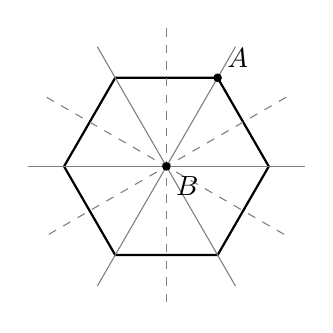
\begin{tikzpicture}[scale=1.3]
\draw[thick] (0:1)--(60:1)--(120:1)--(180:1)--(240:1)--(300:1)--cycle;
\foreach \ang in {0,60,120}
{\draw[gray] (\ang:1.35)--(\ang+180:1.35);}
\foreach \ang in {30,90,150}
{\draw[gray,dashed] (\ang:1.35)--(\ang+180:1.35);}
\fill (0,0) circle (1.2pt) node[below right] {$B$};
\fill (60:1) circle (1.2pt) node[above right] {$A$};
\end{tikzpicture}

\small Solid lines join opposite vertices; dashed lines join
opposite edge midpoints. Both sets are reflection axes.\normalsize
\end{center}

\Needspace{12\baselineskip}
\subsection*{17.2 Representation of Groups}

\Needspace{5\baselineskip}
\par\bigskip
\noindent\textbf{17.2.1}\quad For any representation $K$ of a group,
and for any group element $a$, show that
\[
\big[U^{K}(a)\big]^{-1}=U^{K}\big(a^{-1}\big).
\]
\solution
A matrix representation maps the identity to the identity matrix
and preserves products. Hence
\[
U^K(a)U^K(a^{-1})=U^K(aa^{-1})=U^K(I)=I,
\]
and also
\[
U^K(a^{-1})U^K(a)=U^K(a^{-1}a)=I.
\]
Thus $U^K(a^{-1})$ is both a right and left inverse of $U^K(a)$.
By uniqueness of the matrix inverse,
\[
\boxed{[U^K(a)]^{-1}=U^K(a^{-1})}.
\]
No assumption of a faithful representation or of unitarity is needed.

\Needspace{5\baselineskip}
\par\bigskip
\noindent\textbf{17.2.2}\quad Show that these four matrices form a
representation of the Vierergruppe, whose multiplication table is in
Table~17.2.
\[
\mathsf{I}=\begin{pmatrix}1&0\\0&1\end{pmatrix},\quad
\mathsf{A}=\begin{pmatrix}-1&0\\0&-1\end{pmatrix},\quad
\mathsf{B}=\begin{pmatrix}0&1\\1&0\end{pmatrix},\quad
\mathsf{C}=\begin{pmatrix}0&-1\\-1&0\end{pmatrix}.
\]
\solution
The given matrices obey $A=-I$ and $C=-B$. Direct multiplication gives
\[
B^2=\begin{pmatrix}0&1\\1&0\end{pmatrix}^2=I,
\]
so $A^2=(-I)^2=I$ and $C^2=(-B)^2=I$ as well.
The products of distinct nonidentity matrices are
\[
AB=BA=-B=C,\qquad AC=CA=B,\qquad
BC=CB=-B^2=-I=A.
\]
Multiplication by $I$ leaves every matrix unchanged. These statements
give all 16 products:
\[
\begin{array}{c|cccc}
&I&A&B&C\\\hline
I&I&A&B&C\\
A&A&I&C&B\\
B&B&C&I&A\\
C&C&B&A&I
\end{array}.
\]
The table is exactly Table 17.2; therefore the four matrices form
a representation of the Vierergruppe. Since all four are different,
this particular representation is faithful.

\Needspace{5\baselineskip}
\par\bigskip
\noindent\textbf{17.2.3}\quad Show that the matrices $\mathsf{I}$,
$\mathsf{A}$, $\mathsf{B}$, and $\mathsf{C}$ of Exercise~17.2.2 are
reducible. Reduce them.
\par\emph{Note.}~This means transforming $\mathsf{B}$ and
$\mathsf{C}$ to diagonal form (by the same unitary transformation).
\solution
The eigenvectors of $B$ are
\[
v_+=\frac1{\sqrt2}\binom11,\quad Bv_+=v_+,\qquad
v_-=\frac1{\sqrt2}\binom1{-1},\quad Bv_-=-v_-.
\]
Let $Q=(v_+\ v_-)=2^{-1/2}\begin{pmatrix}1&1\\1&-1\end{pmatrix}$.
Its columns are orthonormal, so $Q^\dagger Q=I$; that is,
$Q^\dagger v_+=(1,0)^T$ and $Q^\dagger v_-=(0,1)^T$.
Since $BQ=(v_+\ \ {-v_-})$, the columns of $Q^\dagger BQ$ are
$(1,0)^T$ and $(0,-1)^T$. Because $C=-B$,
the same eigenvectors diagonalize $C$:
\[
Q^\dagger BQ=\begin{pmatrix}1&0\\0&-1\end{pmatrix},\qquad
Q^\dagger CQ=\begin{pmatrix}-1&0\\0&1\end{pmatrix}.
\]
The scalar matrices $I,A=-I$ are unchanged. Thus the transformed
representation is a direct sum of two one-dimensional representations,
with characters in the order $(I,A,B,C)$
\[
\boxed{(1,-1,1,-1)\quad\text{and}\quad(1,-1,-1,1)}.
\]
Each line $\operatorname{span}\{v_\pm\}$ is invariant under every
group element, proving reducibility and supplying the reduction.

\Needspace{5\baselineskip}
\par\bigskip
\noindent\textbf{17.2.4}
\begin{enumerate}
\item[(a)] Once you have a matrix representation of any group, a 1-D
representation can be obtained by taking the determinants of the
matrices. Show that the multiplicative relations are preserved in
this determinant representation.
\item[(b)] Use determinants to obtain a 1-D representation of
$D_{3}$ from the $2\times2$ representation in Eq.~(17.2).
\end{enumerate}
\solution
\textbf{(a)} If $U(ab)=U(a)U(b)$, the determinant product theorem gives
\[
\chi_{\det}(ab)=\det U(ab)
=\det U(a)\det U(b)=\chi_{\det}(a)\chi_{\det}(b).
\]
Also $\chi_{\det}(I)=1$ and
$\chi_{\det}(a^{-1})=1/\chi_{\det}(a)$.
Every $U(a)$ is invertible, so no determinant is zero.
The determinants therefore define a one-dimensional representation.

\textbf{(b)} In Eq.~(17.2), the matrices of $C_3$ and $C_3^2$
have determinant
$(-1/2)^2+(\sqrt3/2)^2=1$.
The $C_2$ matrix has determinant $-1$; either other twofold matrix
has determinant $(-1/2)(1/2)-(\sqrt3/2)^2=-1$.
Thus
\[
\boxed{\begin{array}{c|rrrrrr}
g&I&C_3&C_3^2&C_2&C_2'&C_2''\\\hline
\chi_{\det}(g)&1&1&1&-1&-1&-1
\end{array}}.
\]
This is the $A_2$ representation of $D_3$.
Products of two flips have determinant $+1$, products of a flip
with a rotation have determinant $-1$, and products of rotations
have determinant $+1$, as required by the group table.

\Needspace{5\baselineskip}
\par\bigskip
\noindent\textbf{17.2.5}\quad Show that the cyclic group of $n$
objects, $C_{n}$, may be represented by $r^{m}$,
$m=0,1,2,\ldots,n-1$. Here $r$ is \erratum{the image of an abstract generator}, given by
\[
r=\exp(2\pi is/n).
\]
The parameter $s$ takes on the values $s=1,2,3,\ldots,n$, with each
value of $s$ yielding a different 1-D (irreducible) representation of
$C_{n}$.
\par\erratum{Take $n\ge1$ and complex representations; the scalar image need not have order $n$.}
\solution
Let $g$ be the abstract generator of $C_n$, so $g^n=I$.
For each integer $s\in\{1,\ldots,n\}$ set
\[
r_s=e^{2\pi is/n},\qquad U_s(g^m)=r_s^m.
\]
Because $r_s^n=e^{2\pi is}=1$, reducing $m$ modulo $n$
does not change this value. For arbitrary integers $j,k$,
\[
U_s(g^jg^k)=r_s^{j+k}=r_s^jr_s^k
=U_s(g^j)U_s(g^k).
\]
Thus this is a representation; it is irreducible since its space
is one-dimensional.

The representations are distinct: equivalence in one dimension
cannot change the scalar $U_s(g)$, and the $n$ numbers
$e^{2\pi is/n}$ are distinct for these $s$.
They are all the irreducible representations. Indeed any complex
representation matrix of $g$ satisfies $U(g)^n=U(g^n)=I$, so its
eigenvalues are $n$th roots of unity; each eigenline is invariant
under every power of $g$. An irreducible representation must
therefore have dimension one. A one-dimensional representation is
fixed by the number $U(g)$, which satisfies $U(g)^n=1$; hence
$U(g)=e^{2\pi is/n}$ for exactly one $s\in\{1,\ldots,n\}$, and the
representation is $U_s$.

\erratum{The scalar $r_s$ is the image of a generator, not
necessarily an element of order $n$. Its order is $n/\gcd(s,n)$.
The representation is faithful only when $\gcd(s,n)=1$;
$s=n$ gives the trivial representation.}
To check the order, $r_s^k=1$ is equivalent to $n$ dividing $sk$.
Write $d=\gcd(s,n)$, $s=ds'$, $n=dn'$; then $n\mid sk$ means
$n'\mid s'k$, and since $\gcd(n',s')=1$ this means $n'\mid k$.
The smallest positive such $k$ is therefore $n'=n/\gcd(s,n)$.

\Needspace{5\baselineskip}
\par\bigskip
\noindent\textbf{17.2.6}\quad Develop the irreducible $2\times2$
matrix representation of the group of rotations (including those that
turn it over) that transform a square into itself. Give the group
multiplication table.
\par\emph{Note.}~This group has the name $D_{4}$ (see Fig.~17.5).
\solution
Take $r$ to be a counterclockwise $90^\circ$ rotation and $s$ a
$180^\circ$ turn about the $x$ axis in the plane of the square.
Their action on in-plane coordinates is
\[
R=\begin{pmatrix}0&-1\\1&0\end{pmatrix},\qquad
S=\begin{pmatrix}1&0\\0&-1\end{pmatrix}.
\]
Thus $R^2=-I$, $R^4=S^2=I$, and
\[
SRS=S(RS)=S\begin{pmatrix}0&1\\1&0\end{pmatrix}
=\begin{pmatrix}0&1\\-1&0\end{pmatrix}=R^{-1}.
\]
The eight matrices, with $U(r^is)=R^iS$, are
\[
\begin{array}{c|cccc}
g&I&r&r^2&r^3\\\hline
U(g)&
\begin{pmatrix}1&0\\0&1\end{pmatrix}&
\begin{pmatrix}0&-1\\1&0\end{pmatrix}&
\begin{pmatrix}-1&0\\0&-1\end{pmatrix}&
\begin{pmatrix}0&1\\-1&0\end{pmatrix}
\end{array},
\]
\[
\begin{array}{c|cccc}
g&s&rs&r^2s&r^3s\\\hline
U(g)&
\begin{pmatrix}1&0\\0&-1\end{pmatrix}&
\begin{pmatrix}0&1\\1&0\end{pmatrix}&
\begin{pmatrix}-1&0\\0&1\end{pmatrix}&
\begin{pmatrix}0&-1\\-1&0\end{pmatrix}
\end{array}.
\]
The first four preserve the displayed side of the square;
the last four turn it over. All are real orthogonal.

Every element is $r^is^\epsilon$, $0\le i<4$, $\epsilon=0,1$.
The relation $srs=r^{-1}$ gives $sr=r^{-1}s$, and applying it
$j$ times, $sr^j=r^{-j}s$. Hence the product rule is
\[
(r^is^\epsilon)(r^js^\eta)
=r^{\,i+(-1)^\epsilon j}s^{\,\epsilon+\eta},
\]
with exponents reduced modulo four and two. This gives the full table
(row times column):
\[
\begin{array}{c|cccccccc}
&I&r&r^2&r^3&s&rs&r^2s&r^3s\\\hline
I&I&r&r^2&r^3&s&rs&r^2s&r^3s\\
r&r&r^2&r^3&I&rs&r^2s&r^3s&s\\
r^2&r^2&r^3&I&r&r^2s&r^3s&s&rs\\
r^3&r^3&I&r&r^2&r^3s&s&rs&r^2s\\
s&s&r^3s&r^2s&rs&I&r^3&r^2&r\\
rs&rs&s&r^3s&r^2s&r&I&r^3&r^2\\
r^2s&r^2s&rs&s&r^3s&r^2&r&I&r^3\\
r^3s&r^3s&r^2s&rs&s&r^3&r^2&r&I
\end{array}.
\]

To prove irreducibility even over $\mathbb C$, a proper nonzero
invariant subspace would be a line. It would have to be an
eigenline of $R$, whose distinct eigenvalues are $i,-i$ with
eigenvectors $(1,-i)^T$ and $(1,i)^T$.
But $S$ interchanges these lines. Neither is invariant under
the whole group, so the two-dimensional representation is irreducible.

\Needspace{12\baselineskip}
\subsection*{17.3 Symmetry and Physics}

\Needspace{5\baselineskip}
\par\bigskip
\noindent\textbf{17.3.1}\quad Consider a quantum mechanics problem
with $D_{3}$ symmetry, with the threefold symmetry axis taken as the
$z$ direction, and with orbitals $\varphi(\mathbf{r}-\mathbf{R}_{j})$
located at the vertices of an equilateral triangle. This is the same
system geometry as in Example~17.3.2, but in the present problem
$\varphi$ will no longer be chosen to have spherical symmetry.
\par Given that $\varphi(\mathbf{r})=(z/r)f(r)$ (so $\varphi$ has the
symmetry of a $p$ orbital oriented along the symmetry axis),
construct linear combinations of the $\varphi$ that are bases for
irreducible representations of $D_{3}$, for each basis indicating its
representation.
\solution
Write $\varphi_j(\mathbf r)=\varphi(\mathbf r-\mathbf R_j)$,
with the vertices numbered cyclically. Use active operations:
$r=C_3$ sends $\varphi_1\to\varphi_2\to\varphi_3\to\varphi_1$.
A twofold rotation $s=C_2$ about the in-plane axis through vertex 1
also reverses $z$. Since each local orbital is proportional to
$z$, its transformation is
\[
s\varphi_1=-\varphi_1,\qquad
s\varphi_2=-\varphi_3,\qquad
s\varphi_3=-\varphi_2.
\]
Thus the sum
\[
\boxed{\psi_{A_2}=\frac{\varphi_1+\varphi_2+\varphi_3}{\sqrt3}}
\]
is unchanged by $r$ and changes sign under $s$.
Its characters on $(I,2C_3,3C_2)$ are $(1,1,-1)$, identifying $A_2$.

Choose two independent zero-sum combinations
\[
u=\frac{2\varphi_1-\varphi_2-\varphi_3}{\sqrt6},\qquad
v=\frac{\varphi_2-\varphi_3}{\sqrt2}.
\]
Substituting $\varphi_1\to\varphi_2\to\varphi_3\to\varphi_1$ gives
\[
ru=\frac{-\varphi_1+2\varphi_2-\varphi_3}{\sqrt6}
=-\frac12u+\frac{\sqrt3}{2}v,\qquad
rv=\frac{\varphi_3-\varphi_1}{\sqrt2}
=-\frac{\sqrt3}{2}u-\frac12v.
\]
The coefficient vectors $(2,-1,-1)/\sqrt6$ and $(0,1,-1)/\sqrt2$ of
$u$ and $v$ are orthonormal, so each coefficient here is an inner
product of coefficient vectors; for example, the coefficient of $v$
in $ru$ is $[0\cdot(-1)+1\cdot2+(-1)(-1)]/\sqrt{12}=\sqrt3/2$.
The substitution for $s$ gives
\[
su=\frac{-2\varphi_1+\varphi_3+\varphi_2}{\sqrt6}=-u,\qquad
sv=\frac{-\varphi_3+\varphi_2}{\sqrt2}=v.
\]
Hence the coefficient matrices in the ordered basis $(u,v)$ are
\[
D_E(r)=\begin{pmatrix}-1/2&-\sqrt3/2\\
\sqrt3/2&-1/2\end{pmatrix},\qquad
D_E(s)=\begin{pmatrix}-1&0\\0&1\end{pmatrix}.
\]
Their traces are $-1$ and $0$, so the characters are $(2,-1,0)$.
An invariant line would have to be an eigenline of $D_E(r)$, whose
distinct eigenvalues $e^{\pm2\pi i/3}$ have eigenvectors
$(1,\mp i)^T$. But $D_E(s)(1,\mp i)^T=-(1,\pm i)^T$, so the flip
interchanges these two lines, and the two-dimensional space is
irreducible. As a check, the representation on
$\operatorname{span}\{\varphi_1,\varphi_2,\varphi_3\}$ has characters
$(3,0,-1)$: $r$ moves every orbital to another site, while $s$
contributes only the diagonal entry $-1$ from $s\varphi_1=-\varphi_1$.
Indeed $(3,0,-1)=(1,1,-1)+(2,-1,0)$. Therefore
\[
\boxed{\operatorname{span}\{\varphi_1,\varphi_2,\varphi_3\}
=A_2\oplus E,\qquad E\text{ has basis }(u,v)}.
\]
\erratum{The Instructor's Manual gives $-I_2$ for a twofold
operation in this $E$ space; that matrix has trace $-2$, whereas
every such operation has eigenvalues $+1,-1$ and trace zero, the
$E$ character, as the direct transformations show.}
The square-root factors normalize the coefficient vectors.
If spatially overlapping orbitals are used, their actual Hilbert-space
norms must be obtained from their overlap integrals; the symmetry
assignments do not depend on those common scale choices.

\Needspace{12\baselineskip}
\subsection*{17.4 Discrete Groups}

\Needspace{5\baselineskip}
\par\bigskip
\noindent\textbf{17.4.1}\quad The Vierergruppe has the multiplication
table shown in Table~17.2.
\begin{enumerate}
\item[(a)] Divide its elements into classes.
\item[(b)] Using the class information, determine for the
Vierergruppe its number of inequivalent irreducible representations
and their dimensions.
\item[(c)] Construct a character table for the Vierergruppe.
\end{enumerate}
\solution
\textbf{(a)} The group is abelian, so
$gag^{-1}=agg^{-1}=a$ for every $a,g$.
Its conjugacy classes are therefore
\[
\boxed{\{I\},\quad\{A\},\quad\{B\},\quad\{C\}}.
\]

\textbf{(b)} The number of inequivalent complex irreducible
representations equals the number of classes, hence is four.
Their positive integer dimensions satisfy
$d_1^2+d_2^2+d_3^2+d_4^2=|\mathcal G|=4$.
Every term is at least one, so each $d_j=1$.

\textbf{(c)} In a one-dimensional representation set
$\chi(A)=a$, $\chi(B)=b$.
Since $A^2=B^2=I$, both $a,b$ are $\pm1$.
The relation $C=AB$ fixes $\chi(C)=ab$.
The four independent choices of $a,b$ give
\[
\boxed{\begin{array}{c|rrrr}
&I&A&B&C\\\hline
A_1&1&1&1&1\\
A_2&1&1&-1&-1\\
A_3&1&-1&1&-1\\
A_4&1&-1&-1&1
\end{array}}.
\]
Each row obeys the multiplication table. Its squared norm
is four, and two distinct rows have two equal and two opposite
entries, giving inner product zero. Thus the table also satisfies
character orthogonality and contains all four irreducibles.

\Needspace{5\baselineskip}
\par\bigskip
\noindent\textbf{17.4.2}\quad The group $D_{3}$ may be discussed as a
permutation group of three objects. Operation $C_{3}$, for instance,
moves vertex 1 to the position formerly occupied by vertex \erratum{3};
likewise vertex 2 moves to the original position of vertex \erratum{1} and
vertex 3 moves to the original position of vertex \erratum{2}. So this
shuffling could be described as the permutation of $(1,2,3)$ to
$(2,3,1)$. Using now letters $a$, $b$, $c$ to avoid notational
confusion, this permutation $(abc)\to(bca)$ corresponds to the matrix
equation
\[
C_{3}\begin{pmatrix}a\\b\\c\end{pmatrix}
=\begin{pmatrix}0&1&0\\0&0&1\\1&0&0\end{pmatrix}
\begin{pmatrix}a\\b\\c\end{pmatrix}
=\begin{pmatrix}b\\c\\a\end{pmatrix},
\]
thereby identifying a $3\times3$ representation of the operation
$C_{3}$.
\begin{enumerate}
\item[(a)] Develop analogous $3\times3$ representations for the other
elements of $D_{3}$.
\item[(b)] Reduce your $3\times3$ representation to the direct sum of
a $1\times1$ and a $2\times2$ representation. Note: This $3\times3$
representation must be reducible or Eq.~(17.10) would be violated.
\end{enumerate}
\par\erratum{The printed statement has vertex 1 moving to the position of vertex 2, vertex 2 to that of vertex 3, and vertex 3 to that of vertex 1, which does not agree with the displayed matrix (see the solution); the vertex motion is reversed here so that the name $C_3$ follows the displayed matrix.}
\solution
\erratum{The printed vertex motion is the active map
$1\to2\to3\to1$. Afterwards position 1 holds the label $c$ of
vertex 3, position 2 holds $a$, and position 3 holds $b$, so it sends
the column of labels at fixed positions from $(a,b,c)$ to $(c,a,b)$.
The displayed matrix instead gives $(b,c,a)$, the inverse reordering.
We retain the displayed matrix for this exercise; using the printed
motion would interchange the labels $C_3$ and $C_3^2$.}

\textbf{(a)} Put
\[
R=\begin{pmatrix}0&1&0\\0&0&1\\1&0&0\end{pmatrix},\qquad
S=\begin{pmatrix}1&0&0\\0&0&1\\0&1&0\end{pmatrix}.
\]
Here $S$ interchanges the second and third entries; as a right
factor it interchanges the second and third columns.
Direct multiplication gives $R^2=U(C_3^2)$ below, $R^3=S^2=I$,
and $SRS=(SR)S=R^{-1}$: interchanging the last two columns of $SR$
(displayed below) gives $R^2=R^T=R^{-1}$.
Hence $R,S$ generate a representation of $D_3$.
The six matrices, named consistently with the multiplication
table $C_2C_3=C_2'$, are
\[
\begin{aligned}
U(I)&=I_3,&
U(C_3)&=R,&
U(C_3^2)&=\begin{pmatrix}0&0&1\\1&0&0\\0&1&0\end{pmatrix},\\
U(C_2)&=S,&
U(C_2')&=SR=\begin{pmatrix}0&1&0\\1&0&0\\0&0&1\end{pmatrix},&
U(C_2'')&=SR^2=\begin{pmatrix}0&0&1\\0&1&0\\1&0&0\end{pmatrix}.
\end{aligned}
\]

\textbf{(b)} All permutations preserve the sum of the three
components. Consequently
\[
e_0=\frac1{\sqrt3}\begin{pmatrix}1\\1\\1\end{pmatrix}
\]
is fixed. The permutation matrices are orthogonal, so its
orthogonal complement, the vectors with zero component sum, is
invariant. Choose an orthonormal basis there:
\[
e_1=\frac1{\sqrt6}\begin{pmatrix}2\\-1\\-1\end{pmatrix},\qquad
e_2=\frac1{\sqrt2}\begin{pmatrix}0\\1\\-1\end{pmatrix},
\qquad Q=(e_0\ e_1\ e_2).
\]
Since $R(a,b,c)^T=(b,c,a)^T$ and $S(a,b,c)^T=(a,c,b)^T$,
\[
Re_1=\frac1{\sqrt6}\begin{pmatrix}-1\\-1\\2\end{pmatrix}
=-\tfrac12e_1-\tfrac{\sqrt3}{2}e_2,\qquad
Re_2=\frac1{\sqrt2}\begin{pmatrix}1\\-1\\0\end{pmatrix}
=\tfrac{\sqrt3}{2}e_1-\tfrac12e_2,
\]
as one checks by adding the right-hand sides componentwise
(note $\tfrac{\sqrt3}{2}e_2=\tfrac{3}{2\sqrt6}(0,1,-1)^T$), and
$Se_1=e_1$, $Se_2=-e_2$. These coefficients form the columns of the
$2\times2$ blocks, while $Re_0=Se_0=e_0$ gives the entry $1$:
\[
Q^\dagger RQ=
1\oplus\begin{pmatrix}-1/2&\sqrt3/2\\-\sqrt3/2&-1/2\end{pmatrix},
\qquad
Q^\dagger SQ=1\oplus\begin{pmatrix}1&0\\0&-1\end{pmatrix}.
\]
Every other group matrix is a product of $R,S$, so the same
$1+2$ block structure holds for all six matrices.
The scalar block is $A_1$; the two-dimensional block has characters
$(2,-1,0)$ and is $E$. Hence
\[
\boxed{U=A_1\oplus E}.
\]
As a check, the traces of $I_3$, $R$, $S$ give the characters
$(3,0,1)$ of $U$ on $(I,2C_3,3C_2)$, and
$(3,0,1)=(1,1,1)+(2,-1,0)$.

\Needspace{5\baselineskip}
\par\bigskip
\noindent\textbf{17.4.3}\quad The group named $D_{4}$ has a fourfold
axis of symmetry, and twofold axes in four directions perpendicular
to the fourfold axis. See Fig.~17.5. $D_{4}$ has the following
classes (the numbers preceding the class descriptors indicate the
number of elements in the class): $I$, $2C_{4}$, $C_{2}$, $2C_{2}'$,
$2C_{2}''$. The twofold axes marked with primes are in the plane of
fourfold symmetry.
\begin{enumerate}
\item[(a)] Find the number and dimensions of the irreducible
representations.
\item[(b)] Given that all the characters of the representations of
dimension 1 are $\pm1$ and that $C_{2}=C_{4}^{2}$, use the
orthogonality conditions to construct a complete character table for
$D_{4}$.
\end{enumerate}
\solution
\textbf{(a)} There are five classes, so there are five irreducible
representations. Their dimensions have squares summing to eight.
No dimension can exceed two, since $3^2=9>8$. If $k$ dimensions are two and
the other $5-k$ are one, then
\[
4k+(5-k)=8\quad\Longrightarrow\quad k=1.
\]
Thus there are four one-dimensional representations and one
two-dimensional representation.

\textbf{(b)} Write the group as
$r^4=s^2=I$, $srs=r^{-1}$, as in 17.2.6.
Its classes are
\[
\{I\},\quad\{r,r^3\},\quad\{r^2\},\quad
\{s,r^2s\},\quad\{rs,r^3s\}.
\]
Indeed, with $sr^j=r^{-j}s$ from 17.2.6, conjugation by $r$ gives
$rsr^{-1}=r^2s$ and $r(rs)r^{-1}=r^3s$, conjugation by $s$ gives
$srs^{-1}=r^{-1}=r^3$, and $r^2$ commutes with every element.
In one dimension, $a=U(r)$ and $b=U(s)$ are scalars.
The relation $bab=a^{-1}$ and $b^2=1$ imply $a=a^{-1}$,
so $a,b=\pm1$. The class characters are therefore
$(1,a,1,b,ab)$, since $\chi(r^2)=a^2=1$ and $\chi(rs)=ab$.
Their four choices give the first four rows below.

For the remaining representation, $\chi_E(I)=2$.
Column orthogonality between a nonidentity column $g$ and the
identity column requires
\[
\sum_K \chi_K(I)^*\chi_K(g)=0.
\]
For $r,r^3$, the first four entries sum to zero, so
$2\chi_E(r)=0$. The same reasoning gives zero on both flip classes.
For $r^2$, the four scalar entries sum to four, so
$4+2\chi_E(r^2)=0$, giving $\chi_E(r^2)=-2$.
Thus the complete table is
\[
\boxed{\begin{array}{c|rrrrr}
D_4&I&2C_4&C_2&2C_2'&2C_2''\\\hline
A_1&1&1&1&1&1\\
A_2&1&1&1&-1&-1\\
B_1&1&-1&1&1&-1\\
B_2&1&-1&1&-1&1\\
E&2&0&-2&0&0
\end{array}}.
\]
Using class weights $(1,2,1,2,2)$, each row has squared norm
eight and distinct rows have inner product zero.
For example $\langle E,E\rangle=4+4=8$, while
$\langle E,A_1\rangle=2-2=0$. This verifies the required
orthogonality; the $E$ matrices in 17.2.6 realize its last row.

\Needspace{5\baselineskip}
\par\bigskip
\noindent\textbf{17.4.4}\quad The eight functions $\pm x^{3}$,
$\pm x^{2}y$, $\pm xy^{2}$, $\pm y^{3}$ \erratum{span a reducible function space} for
$D_{4}$, with $C_{4}$ a $90^{\circ}$ counterclockwise rotation in the
$xy$ plane, $C_{2}=C_{4}^{2}$, $C_{2}'=(x\to -x,\,y\to y)$,
$C_{2}''=(x\to y,\,y\to x)$, and the remaining members of $D_{4}$ are
additional members of the classes containing the above operations.
Find the characters of the reducible representation \erratum{on this span},
and find the direct sum of irreducible representations of which it consists.
\par\erratum{Also distinguish the formal permutation representation on eight independent signed labels, which is the interpretation used by the Instructor's Manual.}
\solution
\erratum{As actual functions, $f$ and $-f$ are linearly dependent.
The eight listed signed functions are not an eight-dimensional
basis: their function space has dimension four. The Instructor's
Manual's eight-dimensional answer describes a different, formal permutation
space whose eight signed labels are treated as independent.
We give both interpretations explicitly.}

For the actual cubic functions take the independent basis
\[
f_1=x^3,\quad f_2=x^2y,\quad f_3=xy^2,\quad f_4=y^3.
\]
Let the quarter-turn act on functions by the substitution
$r:(x,y)\mapsto(y,-x)$, that is, $(rf)(\mathbf r)=f(R^{-1}\mathbf r)$
for the counterclockwise $90^\circ$ rotation $R$. The opposite
convention, $f(R\mathbf r)$, assigns to each operation the matrix of
its inverse; it gives the same characters, because every element of
$D_4$ is conjugate to its inverse. The transformed basis is
\[
r(f_1,f_2,f_3,f_4)=\bigl(y^3,\,y^2(-x),\,y(-x)^2,\,(-x)^3\bigr)
=(f_4,-f_3,f_2,-f_1).
\]
Thus no diagonal coefficient occurs and $\chi(r)=0$.
The half-turn sends every cubic to its negative, so $\chi(r^2)=-4$.
For $s:(x,y)\mapsto(-x,y)$,
\[
s(f_1,f_2,f_3,f_4)=(-f_1,f_2,-f_3,f_4),
\]
whose trace is zero. The diagonal reflection
$(x,y)\mapsto(y,x)$ exchanges $f_1\leftrightarrow f_4$ and
$f_2\leftrightarrow f_3$, again with trace zero. Therefore
\[
\chi_{\rm cubic}=(4,0,-4,0,0)
\quad\text{on }(I,2C_4,C_2,2C_2',2C_2'').
\]
Only $I$ and $C_2$ have nonzero characters, and every
one-dimensional representation has $\chi(C_2)=1$, so the
multiplicity formula $n_K=8^{-1}\sum_{\rm classes}|C|\chi_K^*\chi$ gives
\[
n_{A_1}=n_{A_2}=n_{B_1}=n_{B_2}=\frac{4-4}{8}=0,\qquad
n_E=\frac{4\cdot2+(-4)(-2)}8=2.
\]
Hence the function-space answer is
\[
\boxed{\mathcal P_3=E\oplus E}.
\]
Explicit invariant pairs are $(x^3,y^3)$ and $(x^2y,xy^2)$, as the
transformation lists above show. In each pair a quarter-turn has
eigenvalues $\pm i$:
$r(x^3\mp iy^3)=\pm i(x^3\mp iy^3)$ and
$r(x^2y\pm ixy^2)=\pm i(x^2y\pm ixy^2)$. The reflection $s$
interchanges the eigenlines, since
$s(x^3-iy^3)=-(x^3+iy^3)$ and $s(x^2y+ixy^2)=x^2y-ixy^2$.
Hence neither pair has an invariant line, and each copy is irreducible.

For the formal eight-label interpretation, introduce independent
symbols $e_{j,+},e_{j,-}$ representing the labels $+f_j,-f_j$.
A group operation permutes these eight symbols, so its character
counts fixed labels. The identity fixes eight. The quarter-turn
and diagonal reflection fix none. The half-turn exchanges
each $+$ label with its $-$ partner and fixes none.
The reflection $x\mapsto-x$ fixes the four labels
$\pm x^2y,\pm y^3$. Thus
\[
\chi_{\rm formal}=(8,0,0,4,0),
\]
and
\[
\boxed{\mathcal V_{\rm formal}=2A_1\oplus2B_1\oplus2E}.
\]
Indeed its multiplicities are
$(8+2\cdot4)/8=2$ for $A_1,B_1$,
$(8-2\cdot4)/8=0$ for $A_2,B_2$, and
$(8\cdot2)/8=2$ for $E$.
The map $e_{j,\pm}\mapsto\pm f_j$ commutes with the group action
and maps onto the cubic space; its kernel is spanned by the four
vectors $e_{j,+}+e_{j,-}$. Each operation permutes these kernel
vectors without signs (an operation taking $f_j$ to $\pm f_k$ sends
$e_{j,+}+e_{j,-}$ to $e_{k,+}+e_{k,-}$), so the kernel has characters
$\chi_{\rm formal}-\chi_{\rm cubic}=(4,0,4,4,0)$; the same
multiplicity formula gives $(4+4+2\cdot4)/8=2$ for $A_1,B_1$ and
zero for the others, i.e.\ the kernel is $2A_1\oplus2B_1$.
The quotient by the kernel is the actual cubic function space
$E\oplus E$. This explains why the two legitimate spaces have
different characters and dimensions.

\Needspace{5\baselineskip}
\par\bigskip
\noindent\textbf{17.4.5}\quad The group $C_{4v}$ has a fourfold
symmetry axis in the $z$ direction, reflection symmetries
($\sigma_{v}$) about the $xz$ and $yz$ planes, and additional
reflection symmetries ($\sigma_{d}$, $d=\text{dihedral}$) about
planes that contain the $z$ axis but are $45^{\circ}$ from the $x$
and $y$ axes. See Fig.~17.6. The character table for $C_{4v}$
follows.
\begin{center}
\begin{tabular}{lccccc}
\toprule
& $I$ & $2C_{4}$ & $C_{2}$ & $2\sigma_{v}$ & $2\sigma_{d}$\\
\midrule
$A_{1}$ & 1 & 1 & 1 & 1 & 1\\
$A_{2}$ & 1 & 1 & 1 & $-1$ & $-1$\\
$B_{1}$ & 1 & $-1$ & 1 & 1 & $-1$\\
$B_{2}$ & 1 & $-1$ & 1 & $-1$ & 1\\
$E$ & 2 & 0 & $-2$ & 0 & 0\\
\bottomrule
\end{tabular}
\end{center}
\begin{enumerate}
\item[(a)] Construct the matrix representing one member of each class
of $C_{4v}$ using as a basis a $p_{z}$ orbital at each of the points
$(x,y)=(a,0)$, $(0,a)$, $(-a,0)$, $(0,-a)$, and therefrom extract the
characters of the reducible representation for which these $p_{z}$
orbitals form a basis. A $p_{z}$ orbital has functional form
$(z/r)f(r)$.
\item[(b)] Determine the irreducible representations contained in our
reducible $p_{z}$ representation.
\item[(c)] Form those linear combinations of our $p_{z}$ functions
that are bases for each of the irreducible representations found in
part \erratum{(b)}.
\end{enumerate}
\par\erratum{The printed reference in (c) says (a); the irreducible summands are determined in (b).}
\solution
Let $f_1,f_2,f_3,f_4$ denote the $p_z$ orbitals centered,
in order, at $+x,+y,-x,-y$.
A $C_{4v}$ operation leaves $z$ unchanged, so the local $p_z$
shape incurs no sign change; only the centers are permuted.
We use matrices whose $j$th column gives the image of $f_j$.

\textbf{(a)} Choose $r=C_4$ counterclockwise, $s=\sigma_v$
reflection in the $xz$ plane, and $d=\sigma_d$ reflection in $x=y$.
On the centers, $r$ acts as $+x\to+y\to-x\to-y\to+x$, $r^2$
exchanges opposite centers, $s$ fixes $\pm x$ and exchanges
$+y\leftrightarrow-y$, and $d$ exchanges $+x\leftrightarrow+y$ and
$-x\leftrightarrow-y$. Representatives of the five classes are
therefore
\[
P_I=I_4,\qquad
P_r=\begin{pmatrix}0&0&0&1\\1&0&0&0\\0&1&0&0\\0&0&1&0\end{pmatrix},
\qquad
P_{r^2}=\begin{pmatrix}0&0&1&0\\0&0&0&1\\1&0&0&0\\0&1&0&0\end{pmatrix},
\]
\[
P_s=\begin{pmatrix}1&0&0&0\\0&0&0&1\\0&0&1&0\\0&1&0&0\end{pmatrix},
\qquad
P_d=\begin{pmatrix}0&1&0&0\\1&0&0&0\\0&0&0&1\\0&0&1&0\end{pmatrix}.
\]
The traces are, on $(I,2C_4,C_2,2\sigma_v,2\sigma_d)$,
\[
\boxed{\chi=(4,0,0,2,0)}.
\]
For example $s$ fixes the two orbitals on the $x$ axis,
while $r,r^2,d$ fix none.

\textbf{(b)} With class sizes $(1,2,1,2,2)$,
$n_K=8^{-1}\sum_{\rm classes}|C|\chi_K^*\chi$, in which only the
classes $I$ and $2\sigma_v$ contribute, gives
\[
n_{A_1}=n_{B_1}=\frac{4+2(2)}8=1,\qquad
n_{A_2}=n_{B_2}=\frac{4-2(2)}8=0,\qquad
n_E=\frac{2(4)}8=1.
\]
Thus \(\boxed{\Gamma=A_1\oplus B_1\oplus E}\).

\textbf{(c)} Suitable combinations are
\[
\boxed{\begin{aligned}
A_1:\quad a&=\tfrac12(f_1+f_2+f_3+f_4),\\
B_1:\quad b&=\tfrac12(f_1-f_2+f_3-f_4),\\
E:\quad e_x&=(f_1-f_3)/\sqrt2,\qquad
e_y=(f_2-f_4)/\sqrt2.
\end{aligned}}
\]
Substituting the center permutations gives
\[
ra=a,\quad sa=a,\qquad rb=-b,\quad sb=b,
\]
\[
re_x=e_y,\quad re_y=-e_x,\qquad se_x=e_x,\quad se_y=-e_y,
\qquad de_x=e_y,\quad de_y=e_x.
\]
For instance, $rb=\tfrac12(f_2-f_3+f_4-f_1)=-b$, and
$sb=\tfrac12(f_1-f_4+f_3-f_2)=b$ because $s$ fixes $f_1,f_3$ and
exchanges $f_2,f_4$; also $db=-b$. These generator actions identify
the stated representations. The function $a$ is invariant, as $A_1$
requires. The function $b$ has $\chi(r)=-1$, $\chi(\sigma_v)=1$,
$\chi(\sigma_d)=-1$, which is the $B_1$ row. On $(e_x,e_y)$ the
matrices of $r$ and $s$ are
$\bigl(\begin{smallmatrix}0&-1\\1&0\end{smallmatrix}\bigr)$ and
$\bigl(\begin{smallmatrix}1&0\\0&-1\end{smallmatrix}\bigr)$, the
$E$ matrices of Exercise~17.2.6, with characters $(2,0,-2,0,0)$.
The pair $e_x,e_y$ is odd across the square and transforms like
$(x,y)$.
The four coefficient vectors are mutually orthonormal and hence
independent; their actual function norms, if orbitals overlap,
are handled as explained in 17.3.1.

\Needspace{5\baselineskip}
\par\bigskip
\noindent\textbf{17.4.6}\quad Using the notation and geometry of
Exercise~17.4.5, repeat that exercise for the eight-member basis
consisting of a $p_{x}$ and a $p_{y}$ orbital at each of the points
$(x,y)=(a,0)$, $(0,a)$, $(-a,0)$, $(0,-a)$.
\solution
Write $x_j=p_x(\mathbf r-\mathbf R_j)$ and
$y_j=p_y(\mathbf r-\mathbf R_j)$, with the four sites ordered
as in 17.4.5. All $x_j$ have positive lobe along positive $x$,
and all $y_j$ along positive $y$. The ordered basis is
\[
(x_1,y_1,x_2,y_2,x_3,y_3,x_4,y_4).
\]
Unlike $p_z$, these local orbitals rotate and reflect in their
two-component orientation space.

\textbf{(a)} Let $P_g$ be the site matrix from 17.4.5 and $O_g$
the matrix acting on $(p_x,p_y)$. The operation $g$ carries the
orbital of orientation $p_\alpha$ ($\alpha=x,y$) at site $j$ to the
site $k$ with $(P_g)_{kj}=1$, with orientation
$\sum_\beta(O_g)_{\beta\alpha}\,p_\beta$. Hence
\[
D(g)_{(k,\beta),(j,\alpha)}=(P_g)_{kj}(O_g)_{\beta\alpha},\qquad
\boxed{D(g)=P_g\otimes O_g}.
\]
This formula determines every entry of the requested $8\times8$
matrices. Explicitly, put
\[
R=\begin{pmatrix}0&-1\\1&0\end{pmatrix},\quad
S=\begin{pmatrix}1&0\\0&-1\end{pmatrix},\quad
T=\begin{pmatrix}0&1\\1&0\end{pmatrix},\quad H=I_2.
\]
Because $p_x$ and $p_y$ transform like $x$ and $y$, the orientation
matrices are those of the point operations on $(x,y)$:
$O_r=R$, $O_{r^2}=R^2=-H$, $O_s=S$, $O_d=T$.
In the following block matrices each entry is $2\times2$, and
block $(k,j)$ is $(P_g)_{kj}O_g$:
\[
D(I)=I_8,\qquad
D(r)=\begin{pmatrix}0&0&0&R\\R&0&0&0\\0&R&0&0\\0&0&R&0\end{pmatrix},
\qquad
D(r^2)=\begin{pmatrix}0&0&-H&0\\0&0&0&-H\\-H&0&0&0\\0&-H&0&0\end{pmatrix},
\]
\[
D(s)=\begin{pmatrix}S&0&0&0\\0&0&0&S\\0&0&S&0\\0&S&0&0\end{pmatrix},
\qquad
D(d)=\begin{pmatrix}0&T&0&0\\T&0&0&0\\0&0&0&T\\0&0&T&0\end{pmatrix}.
\]
For example $rx_1=y_2$, $ry_1=-x_2$, $sx_1=x_1$, and
$sy_1=-y_1$, which explain the orientation signs.
The trace of a tensor product is the product of traces,
$\operatorname{tr}(P\otimes O)=\operatorname{tr}P\,\operatorname{tr}O$,
so, class by class,
\[
\chi_D=\chi_{\rm site}\chi_{\rm orientation}
=(4,0,0,2,0)(2,0,-2,0,0)
=\boxed{(8,0,0,0,0)}.
\]

\textbf{(b)} Only the identity contributes to the multiplicity sum:
$n_K=8^{-1}(8)\chi_K(I)=\dim K$.
Therefore
\[
\boxed{\Gamma=A_1\oplus A_2\oplus B_1\oplus B_2\oplus E\oplus E},
\]
with total dimension $4\cdot1+2\cdot2=8$, as required.

\textbf{(c)} The following four combinations give the scalar
representations:
\[
\boxed{\begin{aligned}
A_1:\quad a_1&=(x_1+y_2-x_3-y_4)/2,\\
A_2:\quad a_2&=(y_1-x_2-y_3+x_4)/2,\\
B_1:\quad b_1&=(x_1-y_2-x_3+y_4)/2,\\
B_2:\quad b_2&=(y_1+x_2-y_3-x_4)/2.
\end{aligned}}
\]
They arise from the site pair $(f_1-f_3,f_2-f_4)$ of 17.4.5 and
the orientation pair $(p_x,p_y)$, both of which transform like
$(x,y)$. Written as
\[
\begin{aligned}
a_1&=\tfrac12[(x_1-x_3)+(y_2-y_4)],&
a_2&=\tfrac12[(y_1-y_3)-(x_2-x_4)],\\
b_1&=\tfrac12[(x_1-x_3)-(y_2-y_4)],&
b_2&=\tfrac12[(y_1-y_3)+(x_2-x_4)],
\end{aligned}
\]
they are the scalar product (like $x^2+y^2$), the antisymmetric
product (like the $z$ component $xy'-yx'$ of a cross product), the
difference of diagonal products (like $x^2-y^2$), and
the symmetric off-diagonal product (like $xy$) of the two pairs.
To check them directly, note that with site indices modulo four
\[
r:\ x_j\mapsto y_{j+1},\quad y_j\mapsto-x_{j+1};\qquad
s:\ x_j\mapsto x_{\bar\jmath},\quad y_j\mapsto-y_{\bar\jmath},
\]
where $\bar1=1$, $\bar2=4$, $\bar3=3$, $\bar4=2$. For example,
$ra_1=(y_2-x_3-y_4+x_1)/2=a_1$ and
$sa_1=(x_1-y_4-x_3+y_2)/2=a_1$. In the same way one finds the
eigenvalues under the two generators:
\[
\begin{array}{c|rrrr}
&a_1&a_2&b_1&b_2\\\hline
r&1&1&-1&-1\\
s&1&-1&1&-1
\end{array}.
\]
Since $d=rs$ (as matrices on $(x,y)$, $RS=T$), its eigenvalues
are the corresponding products, so these are exactly the four
character-table rows.

The two independent $E$ pairs are
\[
\boxed{\begin{aligned}
u_x&=(x_1+x_2+x_3+x_4)/2,&
u_y&=(y_1+y_2+y_3+y_4)/2,\\
v_x&=(x_1-x_2+x_3-x_4)/2,&
v_y&=(y_1-y_2+y_3-y_4)/2.
\end{aligned}}
\]
The first pair is the site $A_1$ combination times the orientation
pair; the second uses the site $B_1$ combination.
By the rules above, $ru_x=u_y$, $ru_y=-u_x$, while
$rv_x=(y_2-y_3+y_4-y_1)/2=-v_y$ and
$rv_y=(-x_2+x_3-x_4+x_1)/2=v_x$; also $su_x=u_x$, $su_y=-u_y$,
$sv_x=v_x$, $sv_y=-v_y$. So their generator matrices are
respectively $(R,S)$ and $(-R,S)$. Both have characters
$(2,0,-2,0,0)$ and have no common invariant line: $-R$ has the same
eigenlines $(1,\mp i)^T$ as $R$, and $S$ interchanges them, as in
17.2.6.
The eight coefficient columns displayed above have norm one
and pairwise zero inner products, so they form a complete basis.
As in 17.3.1, coefficient normalization is distinct from spatial
normalization when local orbitals overlap.

\Needspace{12\baselineskip}
\subsection*{17.5 Direct Products}

\Needspace{5\baselineskip}
\par\bigskip
\noindent\textbf{17.5.1}\quad The group $C_{4v}$ has eight elements,
corresponding to the rotational and reflection symmetries of a square
that cannot be turned over. See Fig.~17.6. Symmetry rotations about
the $z$ axis are denoted $C_{4}$, $C_{2}$, $C_{4}'$. Reflections
relative to the $xz$ and $yz$ planes are named $\sigma_{v}$ and
$\sigma_{v}'$; those at $45^{\circ}$ relative to the $xz$ and $yz$
planes are called $\sigma_{d}$ and $\sigma_{d}'$ ($d$ indicates
``dihedral''). The character table for $C_{4v}$ is in Table~17.4.
\begin{enumerate}
\item[(a)] Find the direct sum of irreducible representations of
$C_{4v}$ corresponding to the direct product $E\otimes E$.
\item[(b)] A basis for $E$ (in the context of Fig.~17.5) consists of
the two functions $\varphi_{1}=x$, $\varphi_{2}=y$. Apply a few of
the group operations to this basis and verify the entries for $E$ in
the character table.
\item[(c)] Assume now that we have two sets of variables, $x_{1}$,
$y_{1}$ and $x_{2}$, $y_{2}$, and we form the direct-product basis
$x_{1}x_{2}$, $x_{1}y_{2}$, $y_{1}x_{2}$, $y_{1}y_{2}$. Determine how
the direct-product basis functions can be combined to form bases for
each of the irreducible representations in the direct sum
corresponding to $E\otimes E$.
\end{enumerate}
\solution
\textbf{(a)} For matrices $A,B$,
$\operatorname{tr}(A\otimes B)=(\operatorname{tr}A)(\operatorname{tr}B)$.
The product character is consequently
\[
\chi_{E\otimes E}=(2,0,-2,0,0)^2=(4,0,4,0,0).
\]
For each of the four one-dimensional irreducibles,
$\chi(I)=\chi(C_2)=1$, so its multiplicity is
$(4+4)/8=1$. For $E$ itself it is
$[2(4)+(-2)(4)]/8=0$. Thus
\[
\boxed{E\otimes E=A_1\oplus A_2\oplus B_1\oplus B_2}.
\]

\textbf{(b)} Take $r x=y$, $r y=-x$,
$s x=x$, $s y=-y$, and $d x=y$, $d y=x$.
In the ordered basis $(x,y)$ their coefficient matrices are
\[
D(r)=\begin{pmatrix}0&-1\\1&0\end{pmatrix},\quad
D(r^2)=-I_2,\quad
D(s)=\begin{pmatrix}1&0\\0&-1\end{pmatrix},\quad
D(d)=\begin{pmatrix}0&1\\1&0\end{pmatrix}.
\]
Their traces, together with $\operatorname{tr}I_2=2$, are
$(2,0,-2,0,0)$ as in the $E$ row.

\textbf{(c)} The product basis has independent variables for
particles 1 and 2. Its four convenient combinations are
\[
\boxed{\begin{aligned}
A_1:\quad a_1&=(x_1x_2+y_1y_2)/\sqrt2,\\
A_2:\quad a_2&=(x_1y_2-y_1x_2)/\sqrt2,\\
B_1:\quad b_1&=(x_1x_2-y_1y_2)/\sqrt2,\\
B_2:\quad b_2&=(x_1y_2+y_1x_2)/\sqrt2.
\end{aligned}}
\]
Apply $r$ to each factor: $x_1x_2\to y_1y_2$,
$y_1y_2\to x_1x_2$,
$x_1y_2\to-y_1x_2$, and
$y_1x_2\to-x_1y_2$.
Thus the four eigenvalues of $r$ are $(1,1,-1,-1)$.
Under $s$ a product acquires one minus sign for each $y$,
so the eigenvalues are $(1,-1,1,-1)$.
Under $d$ the two variables are exchanged, giving
$(1,-1,-1,1)$.
These reproduce the four claimed one-dimensional characters.
Their independent coefficient vectors span the full four-dimensional
tensor-product space.

\Needspace{12\baselineskip}
\subsection*{17.6 Symmetric Group}

\Needspace{5\baselineskip}
\par\bigskip
\noindent\textbf{17.6.1}
\begin{enumerate}
\item[(a)] The objects $(abcd)$ are permuted to $(dacb)$. Write out a
$4\times4$ matrix representation of this one permutation.
\par\emph{Hint:}~Compare with Exercise~17.4.2.
\item[(b)] Is the permutation $(abdc)\to(dacb)$ odd or even?
\item[(c)] Is \erratum{either of the permutations in (a) and (b)} a possible member of the $D_{4}$
group, which was the subject of Exercise~17.4.3? Why or why not?
\end{enumerate}
\par\erratum{Keep the two printed inputs distinct. In (c), distinguish the standard cyclic square labeling $1,2,3,4$ from an embedding obtained by relabeling its vertices.}
\solution
\textbf{(a)} The target column selects entries $4,1,3,2$
of the original column:
\[
\boxed{P=\begin{pmatrix}
0&0&0&1\\1&0&0&0\\0&0&1&0\\0&1&0&0
\end{pmatrix}},\qquad
P\begin{pmatrix}a\\b\\c\\d\end{pmatrix}
=\begin{pmatrix}d\\a\\c\\b\end{pmatrix}.
\]
As a map from old positions to new positions, this is
$(1\,2\,4)$ with position 3 fixed. It is a 3-cycle, has
order three, and is even: a 3-cycle is a product of two transpositions.

\textbf{(b)} \erratum{The printed input changes from $(abcd)$
in (a) to $(abdc)$ in (b). These are different permutations.
The manual's answer \emph{even} applies to (a), not to (b) as printed.}
For the literal input $(a,b,d,c)$, the target $(d,a,c,b)$
selects entries $3,1,4,2$. Its matrix is
\[
Q=\begin{pmatrix}
0&0&1&0\\1&0&0&0\\0&0&0&1\\0&1&0&0
\end{pmatrix}.
\]
Its position cycle is $(1\,2\,4\,3)$, which is a product
of three transpositions. Thus the answer to (b) as printed is
\[
\boxed{\text{odd},\qquad \det Q=-1}.
\]
Equivalently the row-selection list $(3,1,4,2)$ has three
inversions, also giving $(-1)^3=-1$.

\textbf{(c)} For the permutation in (a), the answer is unambiguously
$\boxed{\text{no}}$: its order is three, while $D_4$ has only
elements of orders one, two, and four. In particular its order
cannot divide $|D_4|=8$.

\erratum{The original reference in (c) was ambiguous. For the literal
permutation of (b), the geometric labeling must be specified.}
With slots $1,2,3,4$ placed in that cyclic order around the square,
$Q$ is not a symmetry: it sends the adjacent pair $(1,2)$ to
$(2,4)$, a diagonal pair. But a four-cycle is compatible with
an abstract $D_4$ embedding. If the cyclic order of vertices is
chosen to be $1,2,4,3$, then $Q=(1\,2\,4\,3)$ is a quarter-turn.
This distinction resolves the ambiguity without silently changing
the input in (b).

\Needspace{5\baselineskip}
\par\bigskip
\noindent\textbf{17.6.2}
\begin{enumerate}
\item[(a)] The permutation group of four objects, $S_{4}$, has
$4!=24$ elements. Treating the four elements of the cyclic group,
$C_{4}$, as permutations, set up a $4\times4$ matrix representation
of $C_{4}$. Note that $C_{4}$ is a subgroup of \erratum{$S_{4}$}.
\item[(b)] How do you know that this $4\times4$ matrix
representation of $C_{4}$ must be reducible?
\end{enumerate}
\solution
Let $R$ cyclically shift a column of four entries to the left.
The four matrices are
\[
U(I)=I_4,\qquad
U(C_4)=R=\begin{pmatrix}
0&1&0&0\\0&0&1&0\\0&0&0&1\\1&0&0&0
\end{pmatrix},
\]
\[
U(C_4^2)=R^2=\begin{pmatrix}
0&0&1&0\\0&0&0&1\\1&0&0&0\\0&1&0&0
\end{pmatrix},\qquad
U(C_4^3)=R^3=\begin{pmatrix}
0&0&0&1\\1&0&0&0\\0&1&0&0\\0&0&1&0
\end{pmatrix}.
\]
Four shifts restore the original column, so $R^4=I_4$.
The products satisfy $R^jR^k=R^{j+k\pmod4}$, exactly the
cyclic-group law. All four are permutation matrices, so they
form a subgroup of the full permutation group $S_4$
\erratum{(the original note writes $P_4$; this denotes the permutation group $S_4$ just introduced).}

For reducibility, the vector $(1,1,1,1)^T$ is fixed by all
four matrices, giving a proper invariant line.
More fully, let $\omega=i$ and define
\[
v_k=\frac12\begin{pmatrix}1\\\omega^k\\\omega^{2k}\\
\omega^{3k}\end{pmatrix},\qquad k=0,1,2,3.
\]
Cyclic shifting gives $Rv_k=\omega^kv_k$; the last component
works because $\omega^{4k}=1$.
Their inner products are
\[
v_j^\dagger v_k=\frac14\sum_{m=0}^3\omega^{(k-j)m}
=\begin{cases}1,&j=k,\\0,&j\ne k,\end{cases}
\]
by the finite geometric-series formula.
Thus $V=(v_0\,v_1\,v_2\,v_3)$ is unitary and
\[
\boxed{V^\dagger R^mV=\operatorname{diag}(1,i^m,(-1)^m,(-i)^m)}.
\]
The representation reduces to the four one-dimensional irreducible
representations of $C_4$.

\Needspace{5\baselineskip}
\par\bigskip
\noindent\textbf{17.6.3}\quad The permutation group of four objects,
$S_{4}$, has five classes.
\begin{enumerate}
\item[(a)] Determine the number of elements in each class of $S_{4}$
and identify one element of each class as a product of cycles.
\item[(b)] Two of the irreducible representations of $S_{4}$ are of
dimension 1 (and are usually denoted $A_{1}$ and $A_{2}$). Noting
that permutations can be classified as even or odd, find the
characters of $A_{1}$ and $A_{2}$.
\par\emph{Hint.}~Set up a character table and fill in the $A_{1}$ and
$A_{2}$ lines.
\item[(c)] One irreducible representation of $S_{4}$ (usually denoted
$E$) is of dimension 2. Determine the dimensions of all the
irreducible representations of $S_{4}$ other than $A_{1}$, $A_{2}$,
and $E$.
\item[(d)] Complete the character table of $S_{4}$.
\par\emph{Hint.}~Only the even permutations have nonzero characters
in the $E$ representation.
\end{enumerate}
\solution
\textbf{(a)} Conjugation relabels a permutation's cycles and preserves
their lengths. Conversely two permutations with the same cycle
lengths are conjugate by a suitable relabeling. The five possibilities
and their sizes are
\[
\begin{array}{c|c|c}
\text{cycle type}&\text{example}&\text{class size}\\\hline
1+1+1+1&I&1\\
2+1+1&(12)&\binom42=6\\
2+2&(12)(34)&\frac12\binom42=3\\
3+1&(123)&\binom43(3-1)!=8\\
4&(1234)&(4-1)!=6
\end{array}.
\]
For two transpositions, dividing by two removes the ordering
of the two pairs. For a cycle of length $k$, cyclically shifting
its notation describes the same cycle, leaving $k!/k=(k-1)!$
choices. The sizes sum to $24$.

\textbf{(b)} The trivial character is $(1,1,1,1,1)$.
A cycle of length $k$ is a product of $k-1$ transpositions, so
the signs of the five classes are $(1,-1,1,1,-1)$.
These give the $A_1,A_2$ rows below.

\textbf{(c)} There are five irreducibles. The known dimensions
$1,1,2$ account for $1+1+4=6$ of the squared-dimension sum.
The other dimensions $d,e$ obey
$d^2+e^2=24-6=18$. The only positive integer solution is
$d=e=3$.

\textbf{(d)} A useful independent construction supplies the
remaining characters. The ordinary four-dimensional permutation
representation has character equal to its number of fixed letters:
\[
(4,2,0,1,0).
\]
Removing its invariant all-ones line leaves a three-dimensional
representation with character
\[
\chi_{T_2}=(3,1,-1,0,-1).
\]
Its squared character norm is
$9+6(1)+3(1)+8(0)+6(1)=24$, proving irreducibility.
Multiplying by the sign representation gives a second irreducible,
\[
\chi_{T_1}=(3,-1,-1,0,1).
\]
This fixes our names $T_1,T_2$; interchanging their names is
an equally valid convention.

To construct $E$, act on the three pair partitions
\[
12|34,\qquad13|24,\qquad14|23.
\]
The respective numbers of fixed partitions for the five classes
are $(3,1,3,0,1)$. For example $(12)$ fixes $12|34$ and
exchanges the other two; $(12)(34)$ fixes all three; a 3-cycle
cycles all three. A 4-cycle fixes $13|24$ and exchanges the other two.
Remove the all-ones invariant line from this three-dimensional
permutation space to obtain $\chi_E=(2,0,2,-1,0)$.
Its norm is $4+3(4)+8(1)=24$, again proving irreducibility.

The complete table is therefore
\[
\boxed{\begin{array}{c|rrrrr}
S_4&I&6(12)&3(12)(34)&8(123)&6(1234)\\\hline
A_1&1&1&1&1&1\\
A_2&1&-1&1&1&-1\\
E&2&0&2&-1&0\\
T_1&3&-1&-1&0&1\\
T_2&3&1&-1&0&-1
\end{array}}.
\]
Using the displayed class sizes, distinct rows are orthogonal;
for instance $\langle T_1,T_2\rangle=9-6+3-6=0$ and
$\langle E,A_1\rangle=2+6-8=0$.
All five rows have norm squared $24$, and their squared
dimensions sum to $24$, as required.

\Needspace{12\baselineskip}
\subsection*{17.7 Continuous Groups}

\Needspace{5\baselineskip}
\par\bigskip
\noindent\textbf{17.7.1}\quad Determine three $SU(2)$ subgroups of
$SU(3)$.
\solution
Every $SU(2)$ matrix can be written
\[
W=\begin{pmatrix}a&b\\-b^*&a^*\end{pmatrix},
\qquad |a|^2+|b|^2=1.
\]
To see that this describes every such matrix, let its first row be
$(a,b)$, of norm one. Every unit row orthogonal to it has the
form $e^{i\delta}(-b^*,a^*)$. The determinant is then
$e^{i\delta}(|a|^2+|b|^2)=e^{i\delta}$; requiring determinant
one gives $e^{i\delta}=1$. Conversely the displayed matrix has
orthonormal rows and determinant $|a|^2+|b|^2=1$.
Embed this block into each of the three coordinate pairs:
\[
\boxed{\begin{aligned}
H_{12}&=\left\{\begin{pmatrix}a&b&0\\-b^*&a^*&0\\0&0&1\end{pmatrix}\right\},\\
H_{13}&=\left\{\begin{pmatrix}a&0&b\\0&1&0\\-b^*&0&a^*\end{pmatrix}\right\},\\
H_{23}&=\left\{\begin{pmatrix}1&0&0\\0&a&b\\0&-b^*&a^*\end{pmatrix}\right\}.
\end{aligned}}
\]
Each set has the stated constraint on $a,b$.
Products and adjoints act only in the chosen $2\times2$ block,
so each set is a subgroup. Each embedding is injective and
preserves multiplication, making these subgroups isomorphic to
$SU(2)$. They fix, respectively, the third, second, and first basis vector.

For explicit generators, let $E_{ij}$ have a single one in row
$i$, column $j$. In the $(i,j)$ block take
\[
T_x=\frac{E_{ij}+E_{ji}}2,\qquad
T_y=\frac{E_{ij}-E_{ji}}{2i},\qquad
T_z=\frac{E_{ii}-E_{jj}}2.
\]
Using $E_{ab}E_{cd}=\delta_{bc}E_{ad}$, put
$A=E_{ij}$, $B=E_{ji}$, and $D=E_{ii}-E_{jj}$.
Then
\[
[A,B]=D,\qquad [D,A]=2A,\qquad[D,B]=-2B.
\]
Substitution displays all three commutators:
\[
\begin{aligned}
{}[T_x,T_y]&=\frac{[A+B,A-B]}{4i}
=\frac{-2D}{4i}=i\,\frac D2=iT_z,\\
[T_y,T_z]&=\frac{[A-B,D]}{4i}
=\frac{-2(A+B)}{4i}=i\,\frac{A+B}{2}=iT_x,\\
[T_z,T_x]&=\frac{[D,A+B]}4
=\frac{A-B}{2}=i\,\frac{A-B}{2i}=iT_y.
\end{aligned}
\]
In terms of the Gell-Mann matrices, the three triples are
\[
\left(\frac{\lambda_1}2,\frac{\lambda_2}2,\frac{\lambda_3}2\right),
\quad
\left(\frac{\lambda_4}2,\frac{\lambda_5}2,
\frac{\lambda_3+\sqrt3\lambda_8}{4}\right),
\quad
\left(\frac{\lambda_6}2,\frac{\lambda_7}2,
\frac{-\lambda_3+\sqrt3\lambda_8}{4}\right).
\]
\erratum{Equations (17.62) and (17.63) omit a factor $1/2$
in their linear combinations. Direct addition gives
$\sqrt3\lambda_8-\lambda_3=\operatorname{diag}(0,2,-2)$
and $\sqrt3\lambda_8+\lambda_3=\operatorname{diag}(2,0,-2)$.
Their displayed diagonal matrices therefore equal half those
combinations. The generator triples above include the needed factors.}

\Needspace{5\baselineskip}
\par\bigskip
\noindent\textbf{17.7.2}\quad Prove that the matrices $U(n)$
(unitary matrices of order $n$) form a group, and that $SU(n)$ (those
with determinant unity) form a subgroup of $U(n)$.
\solution
Let $U,V$ be $n\times n$ unitary matrices:
$U^\dagger U=UU^\dagger=I_n$ and likewise for $V$.
Their product is unitary because
\[
(UV)^\dagger(UV)=V^\dagger U^\dagger UV
=V^\dagger V=I_n,
\]
and similarly $(UV)(UV)^\dagger=I_n$. Thus $U(n)$ is closed.
Matrix multiplication is associative, $I_n$ is a unitary identity,
and the inverse of $U$ is $U^\dagger$, itself unitary:
$(U^\dagger)^\dagger U^\dagger=UU^\dagger=I_n$.
This proves all group axioms for $U(n)$.

For $SU(n)$, impose $\det U=1$ in addition.
If $U,V\in SU(n)$, then
\[
\det(UV)=\det U\,\det V=1,
\]
so the product is in $SU(n)$. The identity has determinant one,
and $\det U^{-1}=(\det U)^{-1}=1$, so the inverse is in $SU(n)$.
Associativity is inherited from $U(n)$.
Hence \(\boxed{SU(n)\le U(n)}\).
For comparison, unitarity alone gives
$|\det U|^2=\det(U^\dagger U)=1$; restricting this unit-modulus
determinant to the value one is precisely the special-unitary condition.

\Needspace{5\baselineskip}
\par\bigskip
\noindent\textbf{17.7.3}\quad Using Eq.~(17.56) for the matrix
elements of $SU(2)$ corresponding to rotations about the coordinate
axes, find the matrix corresponding to a rotation defined by Euler
angles $(\alpha,\beta,\gamma)$. The Euler angles are defined in
Section~3.4.
\solution
With the Euler convention of Section 3.4, the successive passive
coordinate rotations are about $z$, then the intermediate $y$,
then the final $z$. Equation (17.56) therefore prescribes
\[
U(\alpha,\beta,\gamma)
=e^{i\gamma\sigma_3/2}e^{i\beta\sigma_2/2}e^{i\alpha\sigma_3/2}.
\]
Since $\sigma_j^2=I$, separating even and odd powers of the
exponential gives
$e^{it\sigma_j/2}=I\cos(t/2)+i\sigma_j\sin(t/2)$.
In particular
\[
Z(t)=\begin{pmatrix}e^{it/2}&0\\0&e^{-it/2}\end{pmatrix},
\qquad
Y(\beta)=\begin{pmatrix}\cos(\beta/2)&\sin(\beta/2)\\
-\sin(\beta/2)&\cos(\beta/2)\end{pmatrix}.
\]
First multiply on the right:
\[
Y(\beta)Z(\alpha)=
\begin{pmatrix}
c\,e^{i\alpha/2}&s\,e^{-i\alpha/2}\\
-s\,e^{i\alpha/2}&c\,e^{-i\alpha/2}
\end{pmatrix},
\qquad c=\cos(\beta/2),\ s=\sin(\beta/2).
\]
Left multiplication by $Z(\gamma)$ multiplies its first row by
$e^{i\gamma/2}$ and its second by $e^{-i\gamma/2}$. Hence
\[
\boxed{U(\alpha,\beta,\gamma)=
\begin{pmatrix}
e^{i(\alpha+\gamma)/2}\cos(\beta/2)&
e^{i(\gamma-\alpha)/2}\sin(\beta/2)\\
-e^{i(\alpha-\gamma)/2}\sin(\beta/2)&
e^{-i(\alpha+\gamma)/2}\cos(\beta/2)
\end{pmatrix}}.
\]
Its determinant is $c^2+s^2=1$ and its columns are orthonormal,
so it is in $SU(2)$. This specifies the lift obtained from the
stated exponential product. Changing a single Euler angle by
$2\pi$ changes its sign; the two matrices $U,-U$ correspond
to the same spatial rotation, consistent with the double cover
of $SO(3)$ by $SU(2)$.

\Needspace{5\baselineskip}
\par\bigskip
\noindent\textbf{17.7.4}\quad For a product of three quarks, the
member of $SU(3)$ representation \textbf{10} with
$(I_{3},Y)=\big(\erratum{+\tfrac{3}{2}},1\big)$ is $uuu$.
\begin{enumerate}
\item[(a)] Apply operators in the root diagram for $SU(3)$,
Fig.~17.8, to obtain all the remaining members of the decuplet
comprising the representation \textbf{10}.
\item[(b)] The two representations \textbf{8} can be chosen to have
for $I_{3}=\tfrac{1}{2}$, $Y=1$ the respective members
$\psi_{1}\big(\tfrac{1}{2},1\big)=(ud-du)u$ and
$\psi_{2}\big(\tfrac{1}{2},1\big)=2uud-udu-duu$. Briefly explain why
this choice is possible.
\item[(c)] Using the operators in the root diagram and the above
$\psi_{1}\big(\tfrac{1}{2},1\big)$, find expressions for
$\psi_{1}\big(-\tfrac{1}{2},1\big)$, $\psi_{1}(-1,0)$,
$\psi_{1}(1,0)$, $\psi_{1}\big(-\tfrac{1}{2},-1\big)$, and
$\psi_{1}\big(\tfrac{1}{2},-1\big)$.
\item[(d)] Taking each of the six $\psi_{1}$ functions you now have,
apply an operator that will convert it into $\psi_{1}(0,0)$. Show
that you obtain exactly two linearly independent $\psi_{1}(0,0)$,
thereby justifying the claim that the $\psi_{1}$ are an octet at the
points shown in Fig.~17.10.
\item[(e)] Show that the octet built starting from
$\psi_{2}\big(\tfrac{1}{2},1\big)$ is linearly independent from that
built from $\psi_{1}$.
\item[(f)] Find the wave function $\psi(0,0)$ that is linearly
independent of all the $\psi(0,0)$ functions found in parts
(a)--(e). It is the sole member of the representation \textbf{1}.
\end{enumerate}
\par\erratum{Use the ordered flavor tensor space with $u,d,s$ orthonormal, and the root convention $I_-u=d$, $U_-d=s$, $V_-u=s$ from Fig.~17.8. The conflicting $U,V$ matrix labels in Eq.~(17.67) are corrected below.}
\solution
\erratum{The supplied transcription has $I_3=2/3$ for $uuu$.
The actual textbook (printed p.~861) correctly has $I_3=3/2$:
each $u$ contributes $1/2$. This value is restored in the question.
Also, the matrices labeled $U_\pm$ and $V_\pm$ in Eq.~(17.67)
are interchanged relative to Eqs.~(17.64)--(17.66) and Fig.~17.8.
We use the consistent root-diagram convention below.}

Use an ordered tensor product, so $uds=u\otimes d\otimes s$;
the 27 ordered words are orthonormal.
The single-quark weights and root actions are
\[
u:(1/2,1/3),\qquad d:(-1/2,1/3),\qquad s:(0,-2/3),
\]
\[
I_-u=d,\quad I_+d=u,\qquad
U_-d=s,\quad U_+s=d,\qquad
V_-u=s,\quad V_+s=u,
\]
with all unlisted single-quark actions zero.
On a word the operator acts on all three slots:
\[
T(abc)=(Ta)bc+a(Tb)c+ab(Tc).
\]
Thus the total generators are sums of the three single-slot
generators, not products of them. A word with occupation numbers
$(n_u,n_d,n_s)$ has
\[
I_3=(n_u-n_d)/2,\qquad Y=(n_u+n_d-2n_s)/3.
\]

\textbf{(a) The decuplet.}
Let $\mathcal S(aab)=aab+aba+baa$ for $a\ne b$, and
\[
\mathcal S(uds)=uds+usd+dus+dsu+sud+sdu.
\]
The ten normalized states are
\[
\boxed{\begin{array}{c|c|l}
I_3&Y&\text{state}\\\hline
3/2&1&uuu\\
1/2&1&\mathcal S(uud)/\sqrt3\\
-1/2&1&\mathcal S(ddu)/\sqrt3\\
-3/2&1&ddd\\
1&0&\mathcal S(uus)/\sqrt3\\
0&0&\mathcal S(uds)/\sqrt6\\
-1&0&\mathcal S(dds)/\sqrt3\\
1/2&-1&\mathcal S(ssu)/\sqrt3\\
-1/2&-1&\mathcal S(ssd)/\sqrt3\\
0&-2&sss
\end{array}}.
\]
To derive every coefficient, a symmetric word sum with occupations
$n_a$ has $N=3!/(n_u!n_d!n_s!)$ distinct words.
A root operator changing $a$ into $b$ produces each target word
$n_b+1$ times. The ratio of target and source word counts is
$N'/N=n_a/(n_b+1)$. Therefore its action on normalized sums is
\[
T_{b\leftarrow a}D_{n_u,n_d,n_s}
=\sqrt{n_a(n_b+1)}\,D_{\text{new occupations}}.
\]
For example $I_-uuu=duu+udu+uud=\sqrt3D_{uud}$.
Successive $I_-$ operations down the top row have coefficients
$\sqrt3,2,\sqrt3$.
The remaining rows follow from
\[
\begin{aligned}
V_-D_{uuu}&=\sqrt3D_{uus},&
I_-D_{uus}&=\sqrt2D_{uds},&
I_-D_{uds}&=\sqrt2D_{dds},\\
V_-D_{uus}&=2D_{uss},&
I_-D_{uss}&=D_{dss},&
V_-D_{uss}&=\sqrt3D_{sss}.
\end{aligned}
\]
Here the subscript denotes occupations, so $D_{uss}=D_{ssu}$.
These paths reach all ten states listed. The root actions preserve
complete permutation symmetry; the symmetric three-quark space
has $\binom{3+3-1}{3}=10$ occupation states, so none is omitted.

\textbf{(b) Choosing the two octet highest states.}
At weight $(1/2,1)$ the ordered basis is $(uud,udu,duu)$.
The decuplet coefficient vector is $(1,1,1)/\sqrt3$.
The two proposed vectors have coefficients
\[
a=(0,1,-1),\qquad b=(2,-1,-1).
\]
Their sums are zero, so both are orthogonal to the decuplet.
Also $a\cdot b=-1+1=0$ and their squared norms are $2,6$.
They span the two-dimensional remaining weight space.
Each is annihilated by $I_+$ because its coefficients sum to zero,
and by $U_+,V_+$ because it contains no strange quark.
They can therefore be taken as the two highest states.
The constructions below exhibit all eight states generated from
each, thereby identifying the two octets directly.

\textbf{(c) The six nonzero weights of the first octet.}
Use unnormalized states to keep every replacement visible.
Starting with $A=udu-duu$, the following path gives all requested
weights:
\[
\begin{array}{c|c|l}
\text{state}&(I_3,Y)&\text{word expression and operation}\\\hline
A&(1/2,1)&udu-duu\\
B&(-1/2,1)&I_-A=udd-dud\\
C&(-1,0)&V_-B=sdd-dsd\\
D&(-1/2,-1)&U_-C=sds-dss\\
E&(1/2,-1)&I_+D=sus-uss\\
F&(1,0)&V_+E=suu-usu
\end{array}.
\]
For clarity the first and third steps are
\[
I_-(udu-duu)
=(ddu+udd)-(ddu+dud)=udd-dud,
\]
\[
U_-(sdd-dsd)
=(ssd+sds)-(ssd+dss)=sds-dss.
\]
The remaining steps are equally explicit:
\[
\begin{aligned}
V_-(udd-dud)&=sdd-dsd,\\
I_+(sds-dss)&=sus-uss,\\
V_+(sus-uss)&=(uus+suu)-(uus+usu)=suu-usu.
\end{aligned}
\]
Every listed vector has squared norm two. Dividing them by
$\sqrt2$ produces normalized nonzero-weight states.

\textbf{(d) The two zero-weight states.}
Approach weight $(0,0)$ from each of the six preceding weights.
Define
\[
Z_1=sdu+uds-dsu-dus,\qquad
Z_2=usd+uds-sud-dus.
\]
The complete list of results is
\[
\begin{array}{c|l|c}
\text{operation}&\text{result}&\text{in the }(Z_1,Z_2)\text{ basis}\\\hline
V_-A&sdu+uds-dsu-dus&Z_1\\
U_-B&usd+uds-sud-dus&Z_2\\
I_+C&sud+sdu-usd-dsu&Z_1-Z_2\\
V_+D&uds+sdu-dus-dsu&Z_1\\
U_+E&dus+sud-uds-usd&-Z_2\\
I_-F&sdu+sud-dsu-usd&Z_1-Z_2
\end{array}.
\]
For example $V_-A$ changes either $u$ in each term of
$udu-duu$, giving the four terms in $Z_1$; all six rows
are obtained by the same slot-by-slot rule.
The inner products are
\[
\langle Z_1,Z_1\rangle=\langle Z_2,Z_2\rangle=4,\qquad
\langle Z_1,Z_2\rangle=2.
\]
Their Gram determinant is $16-4=12>0$, so they are independent,
while the table proves that all six incoming results are in their span.
One orthonormal zero-weight pair is
\[
\boxed{z_1=Z_1/2,\qquad z_2=(2Z_2-Z_1)/\sqrt{12}}.
\]
Indeed the second numerator is orthogonal to $Z_1$ and has
norm squared $4(4)+4-4(2)=12$.
The six distinct nonzero weights and these two independent zero
weights supply exactly eight states.

\textbf{(e) Independence of the second octet.}
Interchange slots 1 and 2, calling this unitary operation $P_{12}$.
The first highest state is odd under it:
$P_{12}(udu-duu)=-(udu-duu)$.
The second is even:
$P_{12}(2uud-udu-duu)=2uud-udu-duu$.
Every total root operator commutes with $P_{12}$, because it
sums identical actions on all three slots. Hence all states
generated from the first are odd and all from the second are even.
These eigenspaces are orthogonal: if $P_{12}v=-v$ and
$P_{12}w=w$, then
$\langle v,w\rangle=\langle P_{12}v,P_{12}w\rangle
=-\langle v,w\rangle=0$.

For an explicit check that the second space also has eight states,
use the same path $I_-,V_-,U_-,I_+,V_+$ as in (c):
\[
\begin{array}{c|l}
(I_3,Y)&\psi_2\\\hline
(1/2,1)&2uud-udu-duu\\
(-1/2,1)&dud+udd-2ddu\\
(-1,0)&dsd+sdd-2dds\\
(-1/2,-1)&2ssd-sds-dss\\
(1/2,-1)&2ssu-sus-uss\\
(1,0)&usu+suu-2uus
\end{array}.
\]
For instance lowering the first row gives
$2(dud+udd)-(ddu+udd)-(ddu+dud)=dud+udd-2ddu$.
Applying $V_-$ to its first row and $U_-$ to its second yields
\[
\begin{aligned}
T_1&=2sud+2usd-sdu-uds-dsu-dus,\\
T_2&=sud+dus+usd+uds-2sdu-2dsu.
\end{aligned}
\]
Their Gram matrix is
$\begin{pmatrix}12&6\\6&12\end{pmatrix}$ with determinant
$108>0$, giving two more independent states at zero weight.
The six outer states have norm squared six; a normalized central
pair is $T_1/\sqrt{12}$ and $(2T_2-T_1)/6$.

For completeness, the slot-symmetric subspace under $P_{12}$
has dimension $6\cdot3=18$. Its completely symmetric decuplet
takes ten dimensions, leaving eight. This orthogonal complement
is invariant under $SU(3)$, because both the slot exchange and
full symmetrization commute with $U\otimes U\otimes U$.
The second construction supplies eight independent vectors there
and hence exhausts that invariant complement.
The first octet lies in the nine-dimensional slot-antisymmetric
space; the remaining one-dimensional component is found next.

\textbf{(f) The singlet.}
There are six ordered words at zero weight, in the order
\[
(uds,usd,dus,dsu,sud,sdu).
\]
The decuplet supplies the all-ones vector; the two octets supply
$Z_1,Z_2,T_1,T_2$. These five vectors are independent:
$Z_1,Z_2$ have odd $P_{12}$ parity, while the other three have
even parity; $T_1,T_2$ are independent and each has coefficient
sum zero, so neither their span nor any of its nonzero vectors
is the all-ones line.
The normalized vector orthogonal to all five is
\[
\boxed{\psi_{\mathbf1}
=\frac{uds-usd-dus+dsu+sud-sdu}{\sqrt6}}.
\]
Its coefficients are $(1,-1,-1,1,1,-1)/\sqrt6$.
Their sum is zero, their dot products with $Z_1,Z_2$ are zero,
and orthogonality to $T_1,T_2$ follows also from opposite
$P_{12}$ parity. Its squared norm is one.

Finally this is an invariant state, not merely an unused vector:
it is the fully antisymmetric tensor. Under $U\otimes U\otimes U$
it is multiplied by $\det U=1$ for $U\in SU(3)$.
Equivalently each root operator produces pairs of opposite terms
and annihilates it. Thus it spans the trivial representation.
The first octet starts orthogonal to this invariant singlet and
stays orthogonal under the unitary group action. It therefore fills
the eight-dimensional complement of the singlet within the
nine-dimensional slot-antisymmetric space.

One can also verify irreducibility directly from the displayed
states. In either octet all nonzero outer weights other than the
starting state have a nonzero raising image: use $I_+$ on $B,C$,
$V_+$ on $D$, $U_+$ on $E,F$. At zero weight the replacement
rules give
\[
I_+(aZ_1+bZ_2)=(a-b)F,\qquad
V_+(aZ_1+bZ_2)=(2a+b)A.
\]
Both vanish only if $a=b=0$. The same equations hold with
$Z_j$ replaced by $T_j$ and $A,F$ by the second-octet states.
Thus the common kernel of $I_+,U_+,V_+$ in each octet is exactly
its one-dimensional highest-state line. In the decuplet the
occupation formula shows that any $d$ can be raised by $I_+$
and any $s$ by $V_+$; only $uuu$ is killed by all raising operators.
Every nonzero invariant summand of a finite-dimensional unitary
representation has a highest state. The commuting Hermitian
operators $Y,I_3$ preserve that summand and admit a simultaneous
eigenbasis there. Choose a weight vector of largest $Y$, then
largest $I_3$ among that $Y$ eigenspace. Both $U_+,V_+$ would
increase $Y$, while $I_+$ would increase $I_3$ at the same $Y$;
therefore all three annihilate the chosen vector. Two nonzero orthogonal summands would give
two independent common-kernel vectors, which the preceding
calculations exclude. All three constructed multiplets are
therefore irreducible.

The dimensions and the explicit independent states give
\[
\boxed{\mathbf3\otimes\mathbf3\otimes\mathbf3
=\mathbf{10}\oplus\mathbf8\oplus\mathbf8\oplus\mathbf1},
\qquad 10+8+8+1=27.
\]

\Needspace{12\baselineskip}
\subsection*{17.8 Lorentz Group}

\Needspace{5\baselineskip}
\par\bigskip
\noindent\textbf{17.8.1}\quad Show that in $3+1$ dimensions (this
means three spatial dimension plus time), a boost in the $xy$ plane
at an angle $\theta$ from the $x$ direction has, in coordinates
$(x^{0},x^{1},x^{2},x^{3})$, the generator
\[
\mathsf{S}=i\begin{pmatrix}
0 & \cos\theta & \sin\theta & 0\\
\cos\theta & 0 & 0 & 0\\
\sin\theta & 0 & 0 & 0\\
0 & 0 & 0 & 0
\end{pmatrix}.
\]
\par\erratum{Use $x^0=ct$, metric $\operatorname{diag}(1,-1,-1,-1)$, and $U(\rho)=e^{i\rho S}$ for the passive boost.}
\solution
Let $x^0=ct$ and
$\mathbf n=(\cos\theta,\sin\theta,0)$.
For an infinitesimal passive boost of rapidity $\delta\rho$,
the frame velocity is $c\,\delta\rho\,\mathbf n$ to first order.
Thus
\[
\delta x=-\delta\rho\cos\theta\,x^0,\qquad
\delta y=-\delta\rho\sin\theta\,x^0,\qquad \delta z=0.
\]
Write the most general linear first-order time change as
$\delta x^0=-\delta\rho(ax+by+dz+ex^0)$.
Preservation of $(x^0)^2-x^2-y^2-z^2$ to first order gives
\[
\begin{aligned}
2x^0\delta x^0-2x\delta x-2y\delta y
=2x^0\delta\rho\big[
(\cos\theta-a)x+(\sin\theta-b)y-dz-ex^0\big]=0.
\end{aligned}
\]
Because this polynomial vanishes for every $x,y,z,x^0$, each
coefficient vanishes:
$a=\cos\theta$, $b=\sin\theta$, $d=e=0$. Hence
\[
x'=(I_4-\delta\rho\,B)x+O(\delta\rho^2),\qquad
B=\begin{pmatrix}
0&\cos\theta&\sin\theta&0\\
\cos\theta&0&0&0\\
\sin\theta&0&0&0\\
0&0&0&0
\end{pmatrix}.
\]
The book defines a generator by
$U(\delta\rho)=I_4+i\delta\rho\,S+O(\delta\rho^2)$.
Comparing first-order coefficients, $iS=-B$, so
\[
\boxed{S=iB},
\]
which is the requested generator. With
$\eta=\operatorname{diag}(1,-1,-1,-1)$ one also checks
$B^T\eta+\eta B=0$, the infinitesimal Lorentz condition.

\Needspace{5\baselineskip}
\par\bigskip
\noindent\textbf{17.8.2}
\begin{enumerate}
\item[(a)] Show that the generator in Exercise~17.8.1 produces a
Lorentz transformation matrix for rapidity $\rho$ given by
\[
U(\rho;\theta)=\begin{pmatrix}
\cosh\rho & -\cos\theta\sinh\rho & -\sin\theta\sinh\rho & 0\\
-\cos\theta\sinh\rho & \sin^{2}\theta+\cos^{2}\theta\cosh\rho
& \cos\theta\sin\theta(\cosh\rho-1) & 0\\
-\sin\theta\sinh\rho & \cos\theta\sin\theta(\cosh\rho-1)
& \cos^{2}\theta+\sin^{2}\theta\cosh\rho & 0\\
0 & 0 & 0 & 1
\end{pmatrix}.
\]
\par\emph{Note.}~This transformation matrix is symmetric. All single
boosts (in any spatial direction) have symmetric transformation
matrices.
\item[(b)] Verify that the transformation matrix of part (a) is
consistent with (1) rotating the spatial coordinates to align the
boost direction with a coordinate axis, (2) performing a boost in the
direction of that axis using Eq.~(17.70), and (3) rotating back to
the original coordinate system.
\end{enumerate}
\solution
Put $c_\theta=\cos\theta$, $s_\theta=\sin\theta$, and let $B$
be the real matrix in 17.8.1, so $S=iB$.
Direct multiplication gives
\[
B^2=\begin{pmatrix}
1&0&0&0\\
0&c_\theta^2&c_\theta s_\theta&0\\
0&c_\theta s_\theta&s_\theta^2&0\\
0&0&0&0
\end{pmatrix},\qquad B^3=B,
\]
using $c_\theta^2+s_\theta^2=1$.
Thus every positive odd power is $B$ and every positive even power is
$B^2$. Separating the exponential series,
\[
\begin{aligned}
U(\rho;\theta)=e^{i\rho S}=e^{-\rho B}
&=I_4-B\left(\rho+\frac{\rho^3}{3!}+\cdots\right)
+B^2\left(\frac{\rho^2}{2!}+\frac{\rho^4}{4!}+\cdots\right)\\
&=I_4-B\sinh\rho+B^2(\cosh\rho-1).
\end{aligned}
\]
Writing $C=\cosh\rho$, $H=\sinh\rho$ and inserting the entries yields
\[
\boxed{U(\rho;\theta)=
\begin{pmatrix}
C&-c_\theta H&-s_\theta H&0\\
-c_\theta H&s_\theta^2+c_\theta^2C&c_\theta s_\theta(C-1)&0\\
-s_\theta H&c_\theta s_\theta(C-1)&c_\theta^2+s_\theta^2C&0\\
0&0&0&1
\end{pmatrix}}.
\]
For example the $xx$ entry is
$1+c_\theta^2(C-1)=s_\theta^2+c_\theta^2C$.
The matrix is symmetric. Along the time and $\mathbf n$ directions
it is the $2\times2$ block $\begin{pmatrix}C&-H\\-H&C\end{pmatrix}$;
on the two perpendicular directions it is the identity.
The relation $C^2-H^2=1$ consequently gives both
$U^T\eta U=\eta$ and $\det U=1$.

\textbf{(b)} Rotate the spatial coordinates so that $\mathbf n$
becomes the $x$ direction:
\[
R=\begin{pmatrix}
1&0&0&0\\0&c_\theta&s_\theta&0\\
0&-s_\theta&c_\theta&0\\0&0&0&1
\end{pmatrix},\qquad
U_x=\begin{pmatrix}
C&-H&0&0\\-H&C&0&0\\0&0&1&0\\0&0&0&1
\end{pmatrix}.
\]
First applying $R$, then $U_x$, then $R^{-1}=R^T$ gives
$R^TU_xR$. The first multiplication is
\[
U_xR=
\begin{pmatrix}
C&-Hc_\theta&-Hs_\theta&0\\
-H&Cc_\theta&Cs_\theta&0\\
0&-s_\theta&c_\theta&0\\0&0&0&1
\end{pmatrix}.
\]
Left multiplication by $R^T$ forms
$c_\theta$ times row 2 minus $s_\theta$ times row 3 for
the new $x$ row, and $s_\theta$ times row 2 plus $c_\theta$
times row 3 for the new $y$ row. These are exactly the
two middle rows of the boxed matrix. The other rows are unchanged.
This verifies the rotation--boost--inverse-rotation construction.

\Needspace{5\baselineskip}
\par\bigskip
\noindent\textbf{17.8.3}\quad Obtain the Lorentz transformation
matrix for a boost of finite amount $\rho'$ in the $x$ direction
followed by a finite boost $\rho''$ in the $y$ direction,
\erratum{with both rapidities real and nonzero}. Show that
there are no values of $\rho$ and $\theta$ that can bring this
transformation to the form given in Exercise~17.8.2.
\solution
Write $C'=\cosh\rho'$, $H'=\sinh\rho'$ and similarly
$C'',H''$ for $\rho''$. Since the $x$ boost acts first,
the product is $U_y(\rho'')U_x(\rho')$:
\[
\begin{aligned}
U_yU_x
&=\begin{pmatrix}
C''&0&-H''&0\\0&1&0&0\\-H''&0&C''&0\\0&0&0&1
\end{pmatrix}
\begin{pmatrix}
C'&-H'&0&0\\-H'&C'&0&0\\0&0&1&0\\0&0&0&1
\end{pmatrix}\\
&=\boxed{\begin{pmatrix}
C''C'&-C''H'&-H''&0\\
-H'&C'&0&0\\
-H''C'&H''H'&C''&0\\
0&0&0&1
\end{pmatrix}}.
\end{aligned}
\]
The spatial $xy$ entry is zero, whereas the $yx$ entry is
$H''H'$. For real nonzero $\rho',\rho''$, this product is
nonzero. The matrix is therefore not symmetric.
Every single boost in 17.8.2 is symmetric, so no choice of
$\rho,\theta$ can produce this two-boost matrix.

\erratum{The impossibility statement requires both rapidities
to be nonzero. If $\rho''=0$, the result is the single $x$ boost,
with $\theta=0$ and $\rho=\rho'$. If $\rho'=0$, it is the
single $y$ boost, with $\theta=\pi/2$ and $\rho=\rho''$.
If both vanish, the result is the identity.}

\Needspace{12\baselineskip}
\subsection*{17.9 Lorentz Covariance of Maxwell's Equations}

\Needspace{5\baselineskip}
\par\bigskip
\noindent\textbf{17.9.1}\quad Apply the Lorentz transformation of
Eq.~(17.80) to $F^{\mu\lambda}$ as given in Eq.~(17.79). Verify that
the result is a matrix $F'$ whose elements confirm the results given
in Eqs.~(17.82) and (17.83).
\par\erratum{Take a real boost velocity $|v|<c$, with the metric and passive convention of Exercise~17.8.1.}
\solution
Factor out the common $\varepsilon_0$ in Eq.~(17.79) and use
$\beta=v/c$, $\gamma=(1-\beta^2)^{-1/2}>0$, so $\gamma^2(1-\beta^2)=1$.
The transformation is $F'=UFU^T$; the particular boost matrix
is symmetric, so this is $UFU$, as in Eq.~(17.81).
The first multiplication gives
\[
\frac{UF}{\varepsilon_0}=
\begin{pmatrix}
-\beta\gamma E_z&
-\gamma E_x+\beta\gamma cB_y&
-\gamma E_y-\beta\gamma cB_x&-\gamma E_z\\
E_x&0&-cB_z&cB_y\\
E_y&cB_z&0&-cB_x\\
\gamma E_z&\beta\gamma E_x-\gamma cB_y&
\beta\gamma E_y+\gamma cB_x&\beta\gamma E_z
\end{pmatrix}.
\]
Right multiplication by $U$ mixes only columns 0 and 3.
The six independent entries are therefore
\[
\begin{aligned}
F'^{01}/\varepsilon_0&=-\gamma(E_x-\beta cB_y),&
F'^{02}/\varepsilon_0&=-\gamma(E_y+\beta cB_x),\\
F'^{03}/\varepsilon_0&=(\beta^2\gamma^2-\gamma^2)E_z=-E_z,&
F'^{12}/\varepsilon_0&=-cB_z,\\
F'^{13}/\varepsilon_0&=\gamma(cB_y-\beta E_x),&
F'^{23}/\varepsilon_0&=-\gamma(cB_x+\beta E_y).
\end{aligned}
\]
For instance $F'^{13}/\varepsilon_0$ is row 1 of $UF/\varepsilon_0$
dotted with column 3 of $U$, namely
$E_x(-\beta\gamma)+(cB_y)\gamma$.
The remaining off-diagonal entries are their negatives because
$(UFU^T)^T=UF^TU^T=-UFU^T$; every diagonal entry is zero.

Define
\[
X=\gamma(E_x-\beta cB_y),\quad
Y=\gamma(E_y+\beta cB_x),\quad
P=\gamma(cB_x+\beta E_y),\quad
Q=\gamma(cB_y-\beta E_x).
\]
The entire transformed matrix is
\[
F'=\varepsilon_0
\begin{pmatrix}
0&-X&-Y&-E_z\\
X&0&-cB_z&Q\\
Y&cB_z&0&-P\\
E_z&-Q&P&0
\end{pmatrix}.
\]
Reading it in the same pattern as the original field tensor gives
\[
\boxed{\begin{aligned}
E_x'&=\gamma(E_x-vB_y),&
E_y'&=\gamma(E_y+vB_x),&
E_z'&=E_z,\\
B_x'&=\gamma(B_x+vE_y/c^2),&
B_y'&=\gamma(B_y-vE_x/c^2),&
B_z'&=B_z.
\end{aligned}}
\]
These are precisely Eqs.~(17.82) and (17.83), including their signs.

\Needspace{5\baselineskip}
\par\bigskip
\noindent\textbf{17.9.2}\quad Confirm that the generalization of
Eqs.~(17.82) and (17.83) to a boost corresponding to an arbitrary
velocity \erratum{$\mathbf v$ with $|\mathbf v|<c$} is properly given by Eq.~(17.84).
\par\erratum{At $\mathbf v=0$, interpret the direction-dependent projections through the continuous zero-velocity limit.}
\solution
For $0<|\mathbf v|<c$, put
$\mathbf n=\mathbf v/|\mathbf v|$ and $\gamma=(1-|\mathbf v|^2/c^2)^{-1/2}$.
Split the fields into
parallel and perpendicular parts:
\[
\mathbf E_\parallel=(\mathbf E\cdot\mathbf n)\mathbf n,\quad
\mathbf E_\perp=\mathbf E-\mathbf E_\parallel,\qquad
\mathbf B_\parallel=(\mathbf B\cdot\mathbf n)\mathbf n,\quad
\mathbf B_\perp=\mathbf B-\mathbf B_\parallel.
\]
Choose a proper spatial rotation taking $\mathbf n$ to the
$z$ axis. In those coordinates 17.9.1 says that the longitudinal
components do not change, while the transverse electric components
are $\gamma(E_x-vB_y,E_y+vB_x)$.
These are exactly
$\gamma(\mathbf E_\perp+\mathbf v\times\mathbf B)$.
Likewise the transverse magnetic components are
$\gamma(\mathbf B_\perp-\mathbf v\times\mathbf E/c^2)$.
Proper rotations preserve dot and cross products, so these vector
statements remain valid after rotating back.

Adding the unchanged longitudinal parts gives
\[
\begin{aligned}
\mathbf E'
&=\mathbf E_\parallel+
\gamma(\mathbf E-\mathbf E_\parallel+\mathbf v\times\mathbf B)\\
&=\boxed{\gamma(\mathbf E+\mathbf v\times\mathbf B)
+(1-\gamma)\mathbf E_\parallel},\\
\mathbf B'
&=\mathbf B_\parallel+
\gamma(\mathbf B-\mathbf B_\parallel-\mathbf v\times\mathbf E/c^2)\\
&=\boxed{\gamma(\mathbf B-\mathbf v\times\mathbf E/c^2)
+(1-\gamma)\mathbf B_\parallel}.
\end{aligned}
\]
These are Eq.~(17.84), with $\mathbf E_\parallel=\mathbf E_v$,
$\mathbf B_\parallel=\mathbf B_v$.

\erratum{At $\mathbf v=0$ the direction $\hat{\mathbf v}$ is
undefined; the equations mean their continuous limit,
$\mathbf E'=\mathbf E$, $\mathbf B'=\mathbf B$.}
An equivalent form makes this endpoint explicit. Since
$\gamma^2-1=\gamma^2v^2/c^2$,
\[
\frac{\gamma-1}{v^2}=\frac{\gamma^2}{(\gamma+1)c^2}.
\]
Thus, for all $|\mathbf v|<c$, including zero,
\[
\boxed{\begin{aligned}
\mathbf E'&=\gamma(\mathbf E+\mathbf v\times\mathbf B)
-\frac{\gamma^2}{\gamma+1}\frac{\mathbf v(\mathbf v\cdot\mathbf E)}{c^2},\\
\mathbf B'&=\gamma(\mathbf B-\mathbf v\times\mathbf E/c^2)
-\frac{\gamma^2}{\gamma+1}\frac{\mathbf v(\mathbf v\cdot\mathbf B)}{c^2}.
\end{aligned}}
\]
Both the longitudinal invariance and the $z$-boost component
formulas follow immediately from this expression.

